\documentclass{article}
\usepackage{xeCJK}
\usepackage{amsmath}
\usepackage{amssymb}
\usepackage{mathrsfs}
\usepackage{bm}
\usepackage{hyperref}
\usepackage{graphicx}
\usepackage{subcaption}
\usepackage{float}
\usepackage{multicol}
\usepackage[ruled,linesnumbered]{algorithm2e}

\setlength{\parindent}{2em}
\usepackage{geometry}
\geometry{a4paper, left=2.54cm, right=2.54cm, top=3.18cm, bottom=3.18cm}

% 设置文章行距
\renewcommand{\baselinestretch}{1.5}

% 定义引用格式
% \newcommand{\myeqref}[1]{\eqref{#1}式}
% \newcommand{\figref}[1]{图\ref{#1}}
% \newcommand{\tabref}[1]{表\ref{#1}}

\begin{document}

\section{模型}

\begin{eqnarray}
    \dot{x}_i&=&v\cos \theta _i\;,\label{eq:dotxi}
  \\
    \dot{y}_i&=&v\sin \theta _i\;,\label{eq:dotyi}
  \\
    \dot{\theta}_i&=&\omega _i+\lambda \sum_{j=1}^N{A_{ij}\sin \left( \theta _j-\theta _i \right)}
    \label{eq:dotthetai}
\end{eqnarray}
其中
\begin{equation}
    A_{ij}=\begin{cases}
        1,&		\left| \mathbf{r}_i-\mathbf{r}_j \right|\le d_0\\
        0,&		\left| \mathbf{r}_i-\mathbf{r}_j \right|>d_0\\
    \end{cases}
\end{equation}
$\left| \mathbf{r}_i-\mathbf{r}_j \right|$为振子$i$与振子$j$之间的欧氏距禂, $d_0$为振子的作用半径. $\omega _i$为振子$i$的自然频率, $\lambda$为耦合强度, $v$为振子的运动速度.

为方便研究,考虑到周期性边界条件

\begin{equation}
    \begin{array}{c}
        x_i\left( t+\Delta t \right) =x_i\left( t \right) +v\cos \theta _i\left( t \right) \Delta t\,\,\mathrm{mod}\ L,\\
        x_i\left( t+\Delta t \right) =x_i\left( t \right) +v\cos \theta _i\left( t \right) \Delta t\,\,\mathrm{mod}\ L,\\
    \end{array}
\end{equation}
考虑周期性边界后,原始的欧氏距离对边界两侧的振子(如\ref{fig:fig1}中A,B,C,D点)失真,因此需要对跨边界的坐标进行调整. 

\subsection{局部耦合中跨边界坐标的调整}\label{positionAdj}

\begin{figure}[htbp]
    \centering
    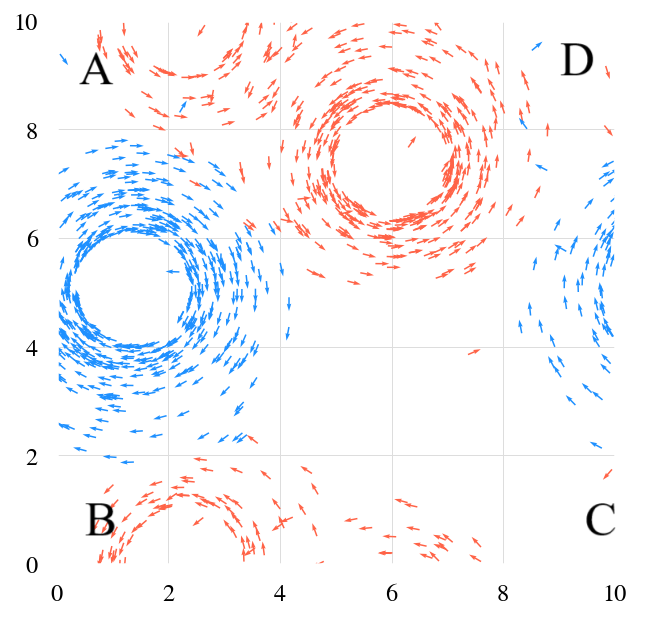
\includegraphics[width=0.4\textwidth]{./figs/fig1.jpg}
    \caption{跨边界坐标的调整}
    \label{fig:fig1}
\end{figure}

给定$(x_i, y_i)$, 对于任意的$(x_j, y_j)$, 做如下变换

\begin{equation}\label{eq:eq1}
	\bar{x}_j=\begin{cases}
		x_j,&		|x_i-x_j|\le L/2\\
		x_j+L,&		x_i-x_j>L/2\\
		x_j-L,&		x_j-x_i>L/2\\
	\end{cases} ,\quad
	\bar{y}_j=\begin{cases}
		y_j,&		|y_i-y_j|\le L/2\\
		y_j+L,&		y_i-y_j>L/2\\
		y_j-L,&		y_j-y_i>L/2\\
	\end{cases}
\end{equation}

其中,$L$为边界长度. 例如,对于\ref{fig:fig1}中的情况,以A为$(x_i, y_i)$时,B需调整纵坐标,D需调整横坐标,C需同时调整横纵坐标.

$\ $

原始距离为

$$
d_{ij}=\sqrt{(x_i-x_j)^2+(y_i-y_j)^2}
$$

变换后的距离为

$$
\bar{d}_{ij}=\sqrt{(x_i-\bar{x}_j)^2+(y_i-\bar{y}_j)^2}
$$

下证$\bar{d}_{ij} \le d_{ij}$, 即调整后的距离不会大于原始距离.

$ $

对于$(x_i-x_j)^2, (x_i-\bar{x}_j)^2$, 若$x_i\ne \bar{x}_j$,有

$$
\begin{array}{l}
	(x_i-\bar{x}_j)^2-(x_i-x_j)^2\\
	=\left( x_j\pm L-x_i \right) ^2-(x_i-x_j)^2\\
	=L^2\pm 2L\left( x_j-x_i \right)\\
	=\left\{ \begin{matrix}
	L^2+2L\left( x_j-x_i \right) ,&		x_i-x_j>5\\
	L^2-2L\left( x_j-x_i \right) ,&		x_j-x_i>5\\
\end{matrix} \right.\\
	<L^2-10L\\
	=0, \left( L=10 \right)\\
\end{array}
$$

即

$$
(x_i-\bar{x}_j)^2<(x_i-x_j)^2, \left( L=10, x_i\ne \bar{x}_j \right)
$$

同理可证

$$
(y_i-\bar{y}_j)^2<(y_i-y_j)^2, \left( L=10, x_i\ne \bar{x}_j \right)
$$

综上有

$$
\bar{d}_{ij}=\sqrt{(x_i-\bar{x}_j)^2+(y_i-\bar{y}_j)^2}\le \sqrt{(x_i-x_j)^2+(y_i-y_j)^2}=d_{ij}
$$

当且仅当$x_i=\bar{x}_j$且$y_i=\bar{y}_j$时,取等号.

因此

$$
\begin{aligned}
	D_{ij}&=\min \left\{ \sqrt{(x_i-\bar{x}_j)^2+(y_i-\bar{y}_j)^2},\sqrt{(x_i-x_j)^2+(y_i-y_j)^2} \right\}\\
	&=\sqrt{(x_i-\bar{x}_j)^2+(y_i-\bar{y}_j)^2}\\
\end{aligned}
$$

\newpage
\section{数值模拟结果}
\begin{figure}[H]
	\centering
	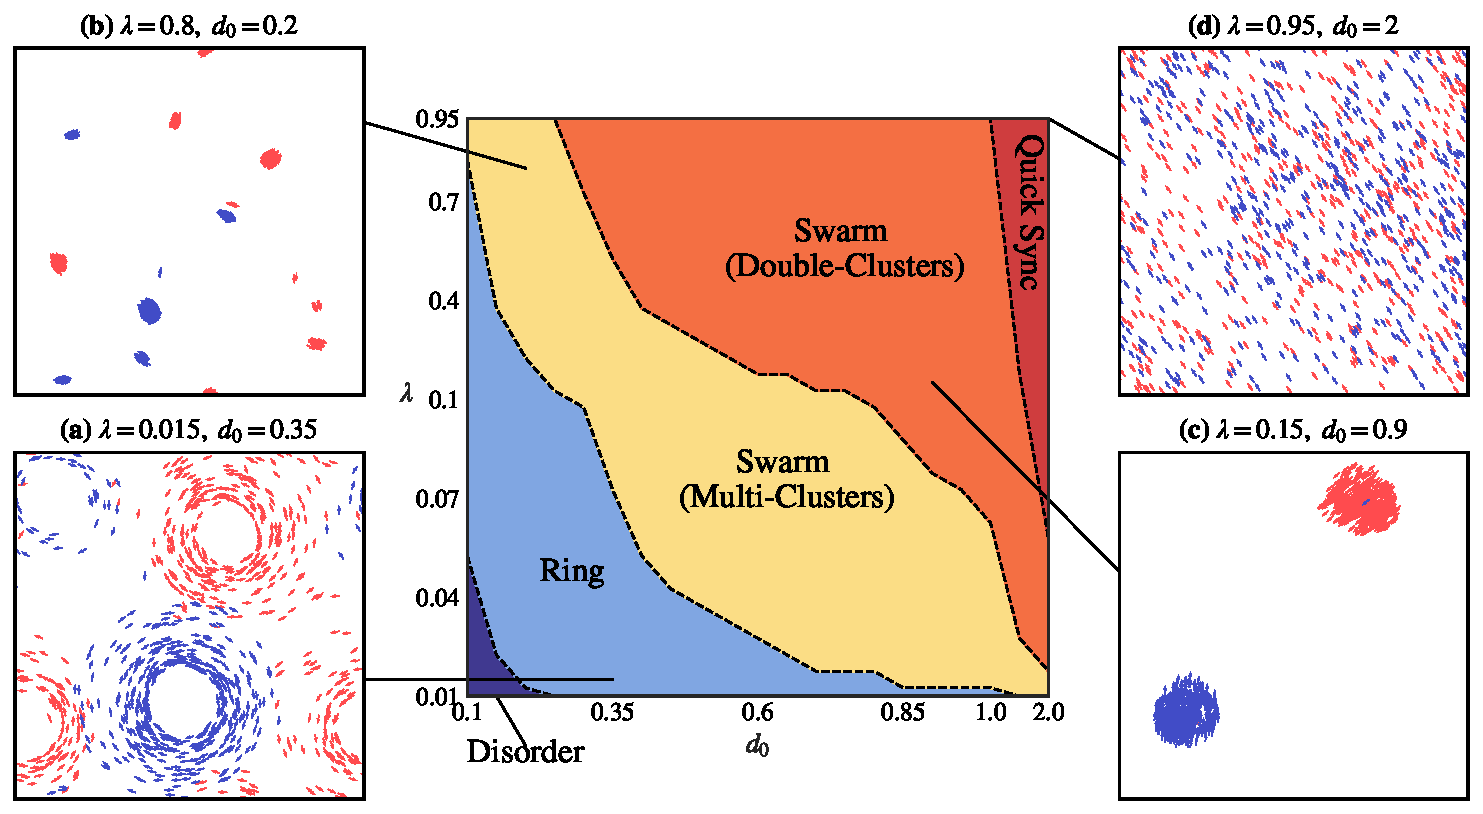
\includegraphics[width=\textwidth]{./figs/phaseDiagram.pdf}
	\caption{相图}
\end{figure}

\subsubsection{相位单位圆}

由于振子数较多,为了更清晰地刻画振子相位的同步情况,绘制三维空间中的单位圆. 将单位圆等分为$M$个区间,每个区间的大小为$\frac{2\pi}{M}$,$z$轴表示单位圆上相位处于该区间的振子数,类似于分布.

\begin{figure}[H]
	\centering
	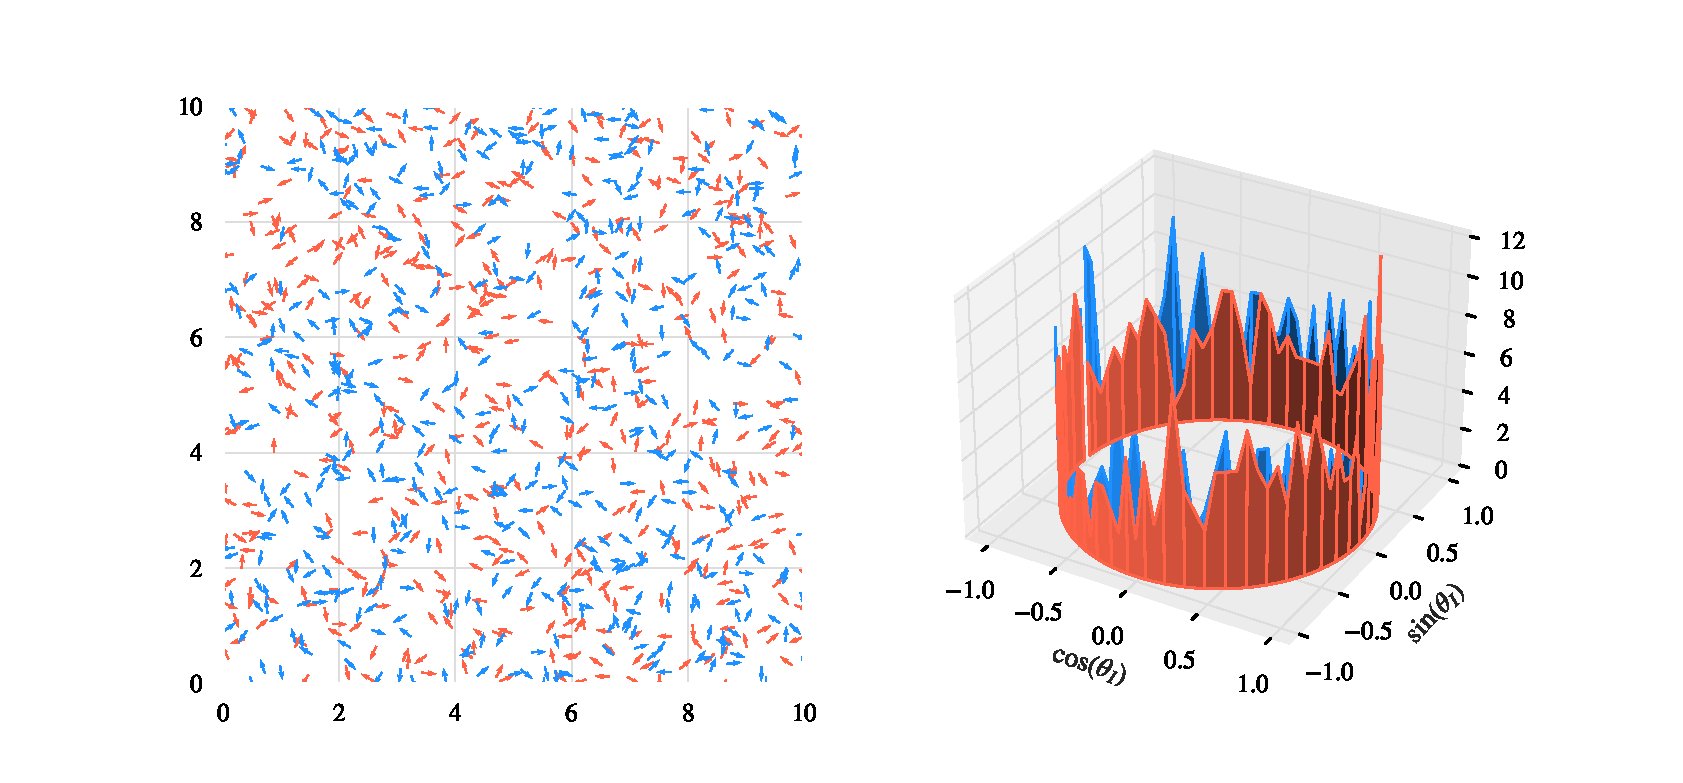
\includegraphics[width=\textwidth]{./figs/CorrectCoupling_uniform_0.010_0.10.eps}
	\vspace{-1cm}
	\caption{无序态 ($\lambda=0.01, d_0=0.1, random seed=10$)}
	\label{fig:fig231.1}
\end{figure}

\begin{figure}[H]
	\centering
	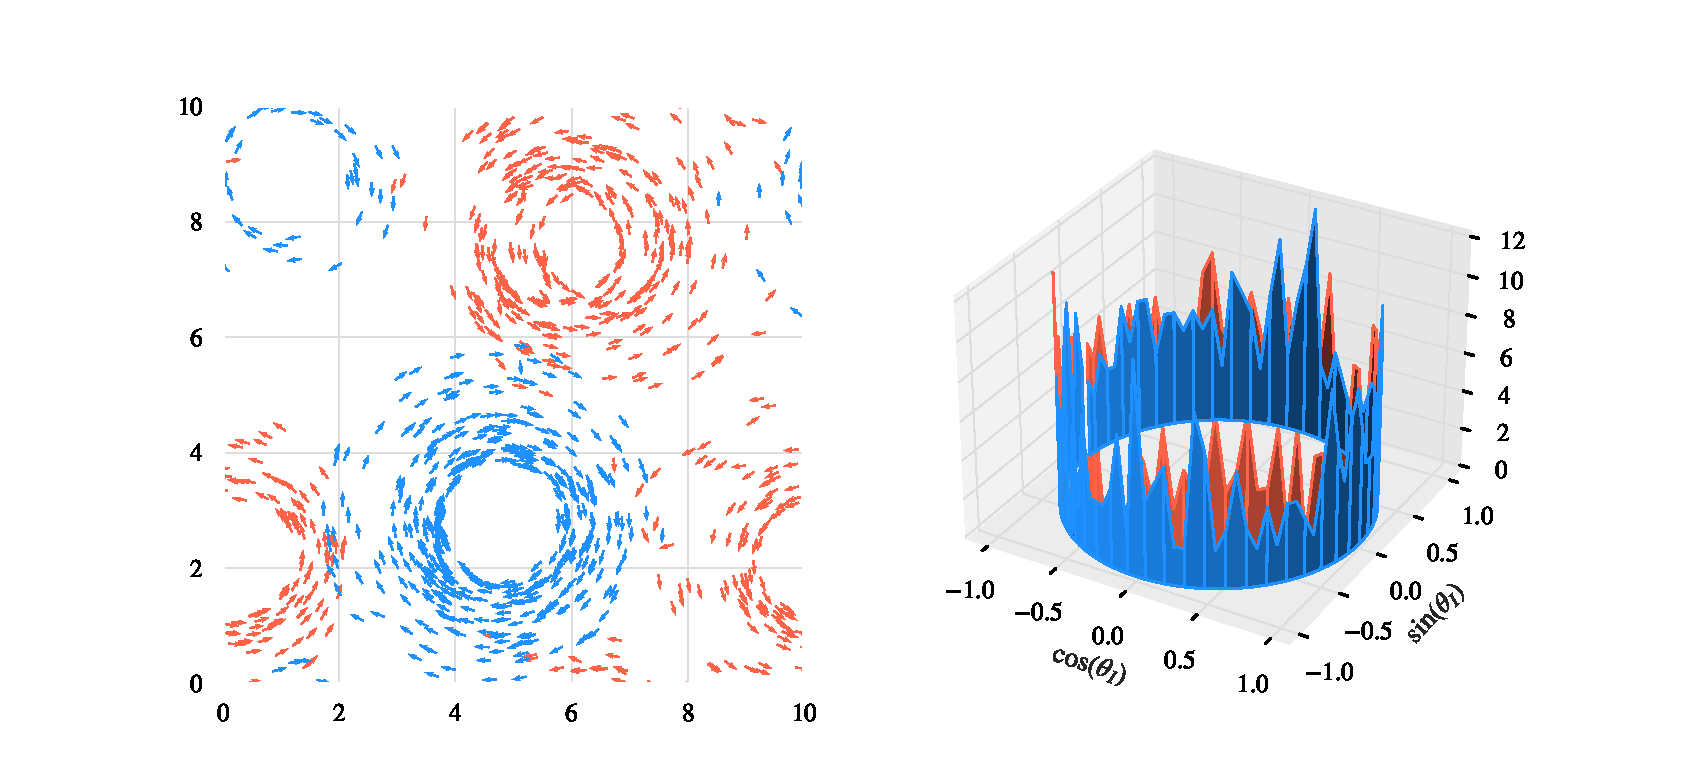
\includegraphics[width=\textwidth]{./figs/CorrectCoupling_uniform_0.020_0.30.eps}
	\vspace{-1cm}
	\caption{环态 ($\lambda=0.02, d_0=0.3, random seed=10$)}
	\label{fig:fig231.2}
\end{figure}

当振子处于无序态或环态时,相位单位圆的分布如图\ref{fig:fig231.1}和图\ref{fig:fig231.2}所示. 此时,单位圆分布较为平滑,单位圆上的振子数分布较为均匀, 相位同步的程度较低.

\begin{figure}[H]
	\centering
	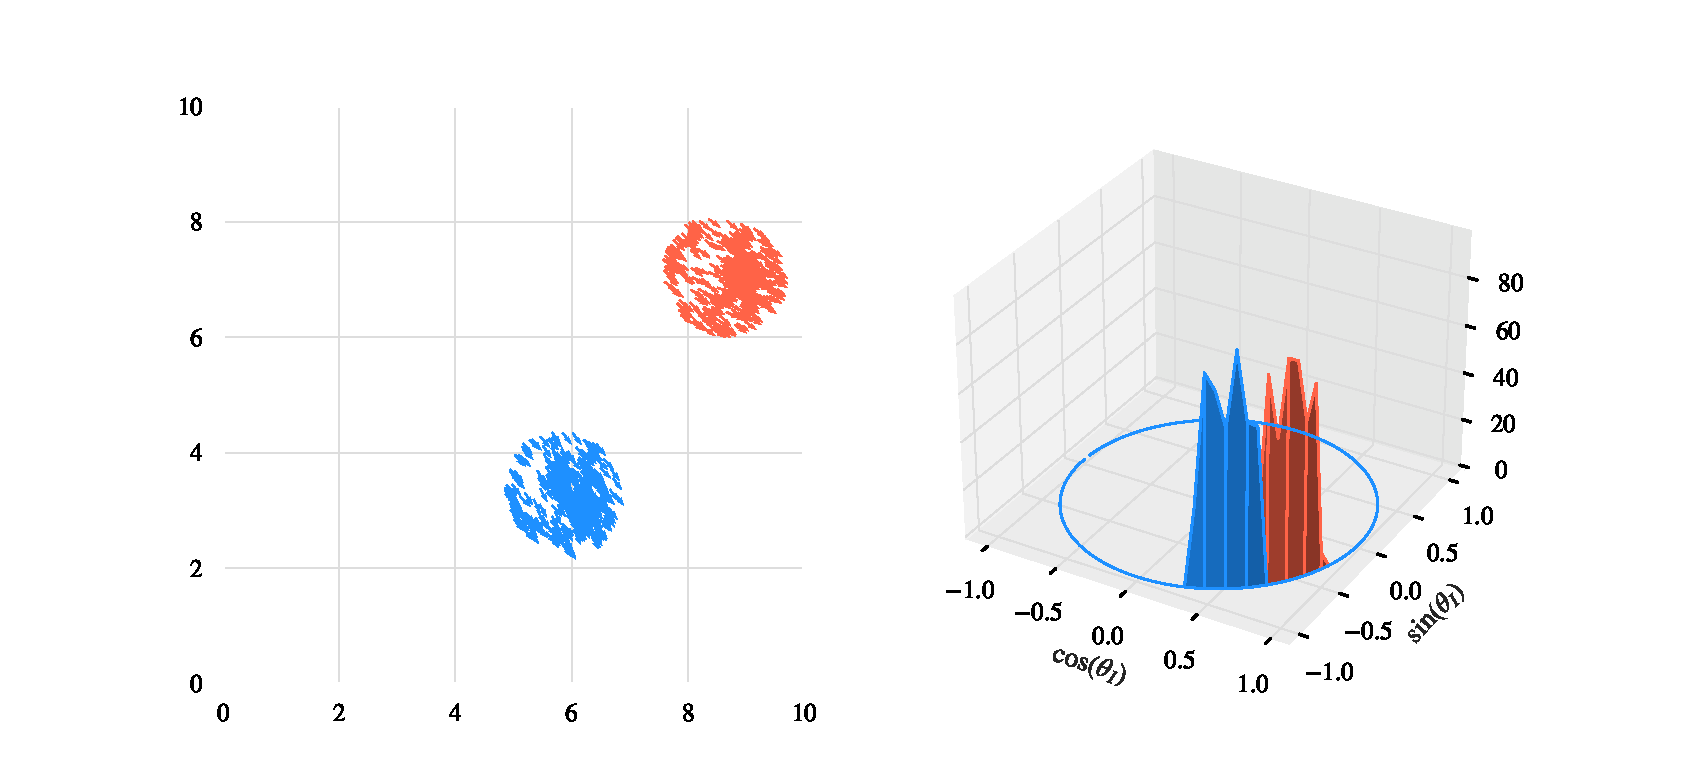
\includegraphics[width=\textwidth]{./figs/CorrectCoupling_uniform_0.010_2.00.eps}
	\vspace{-1cm}
	\caption{集群态 ($\lambda=0.01, d_0=2, random seed=10$)}
	\label{fig:fig231.3}
\end{figure}

\begin{figure}[H]
	\centering
	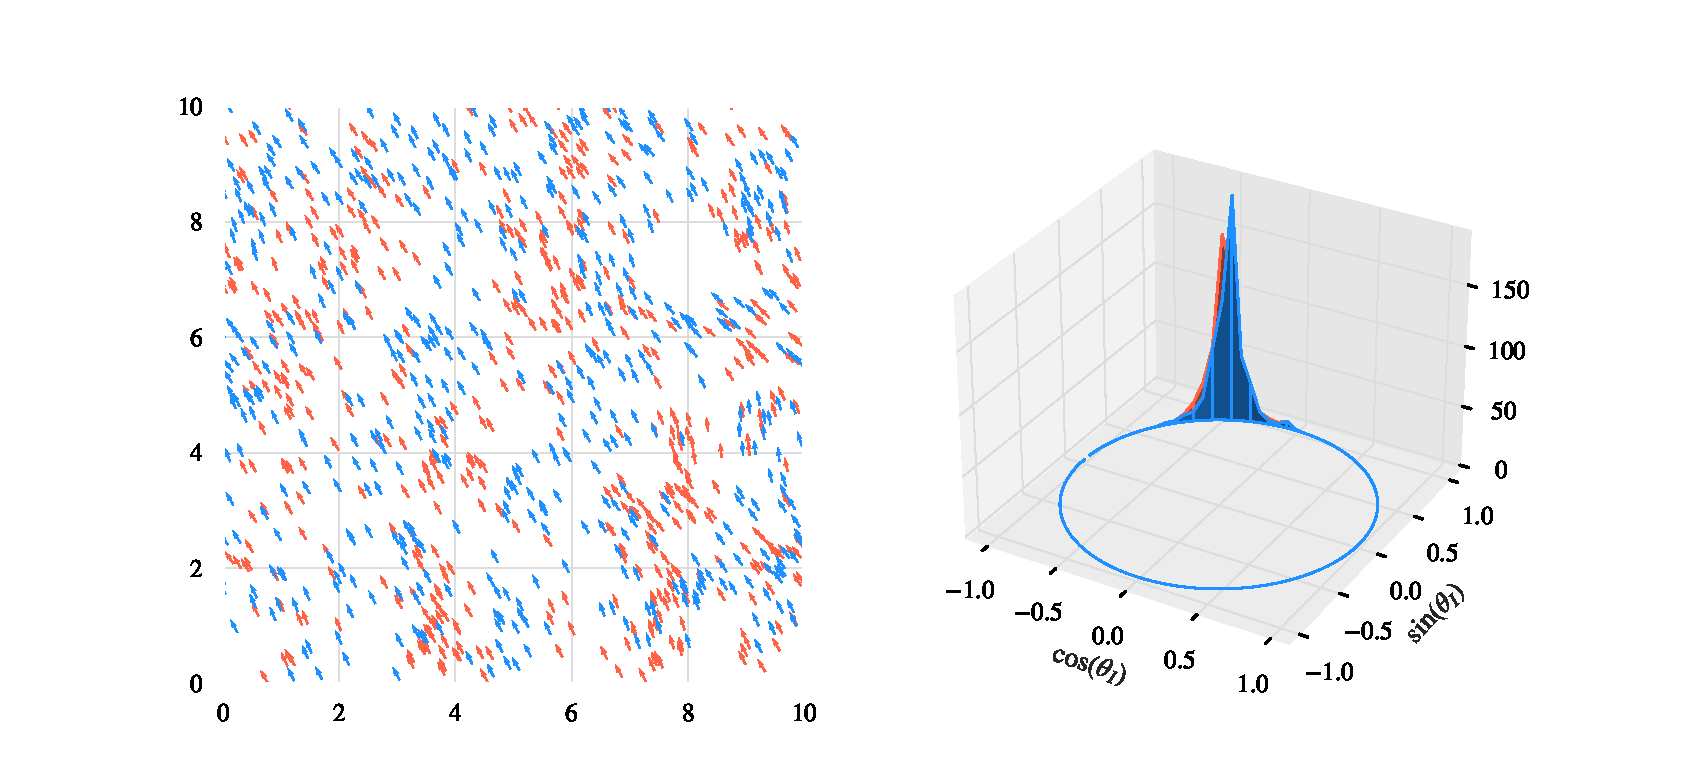
\includegraphics[width=\textwidth]{./figs/CorrectCoupling_uniform_0.600_3.00.eps}
	\vspace{-1cm}
	\caption{瞬时同步态 ($\lambda=0.6, d_0=3, random seed=10$)}
	\label{fig:fig231.4}
\end{figure}

当振子处于集群态或瞬时同步态时,相位单位圆的分布如图\ref{fig:fig231.3}和图\ref{fig:fig231.4}所示. 这两种状态的相位同步的程度较高.

% \begin{enumerate}
%     \item 环态及其相变——无序态、环态、集群态
%     \item 环态的解域与相位同步的关系——局部锁相
%     \item 数值结果的细致讨论, 分类——序参量、旋转半径和中心、聚集与排斥
%     \item 必要的理论分析与估计——四条临界耦合强度线的求解
% \end{enumerate}

\subsubsection{振子旋转中心的坐标}

\begin{figure}[H]
	\centering
	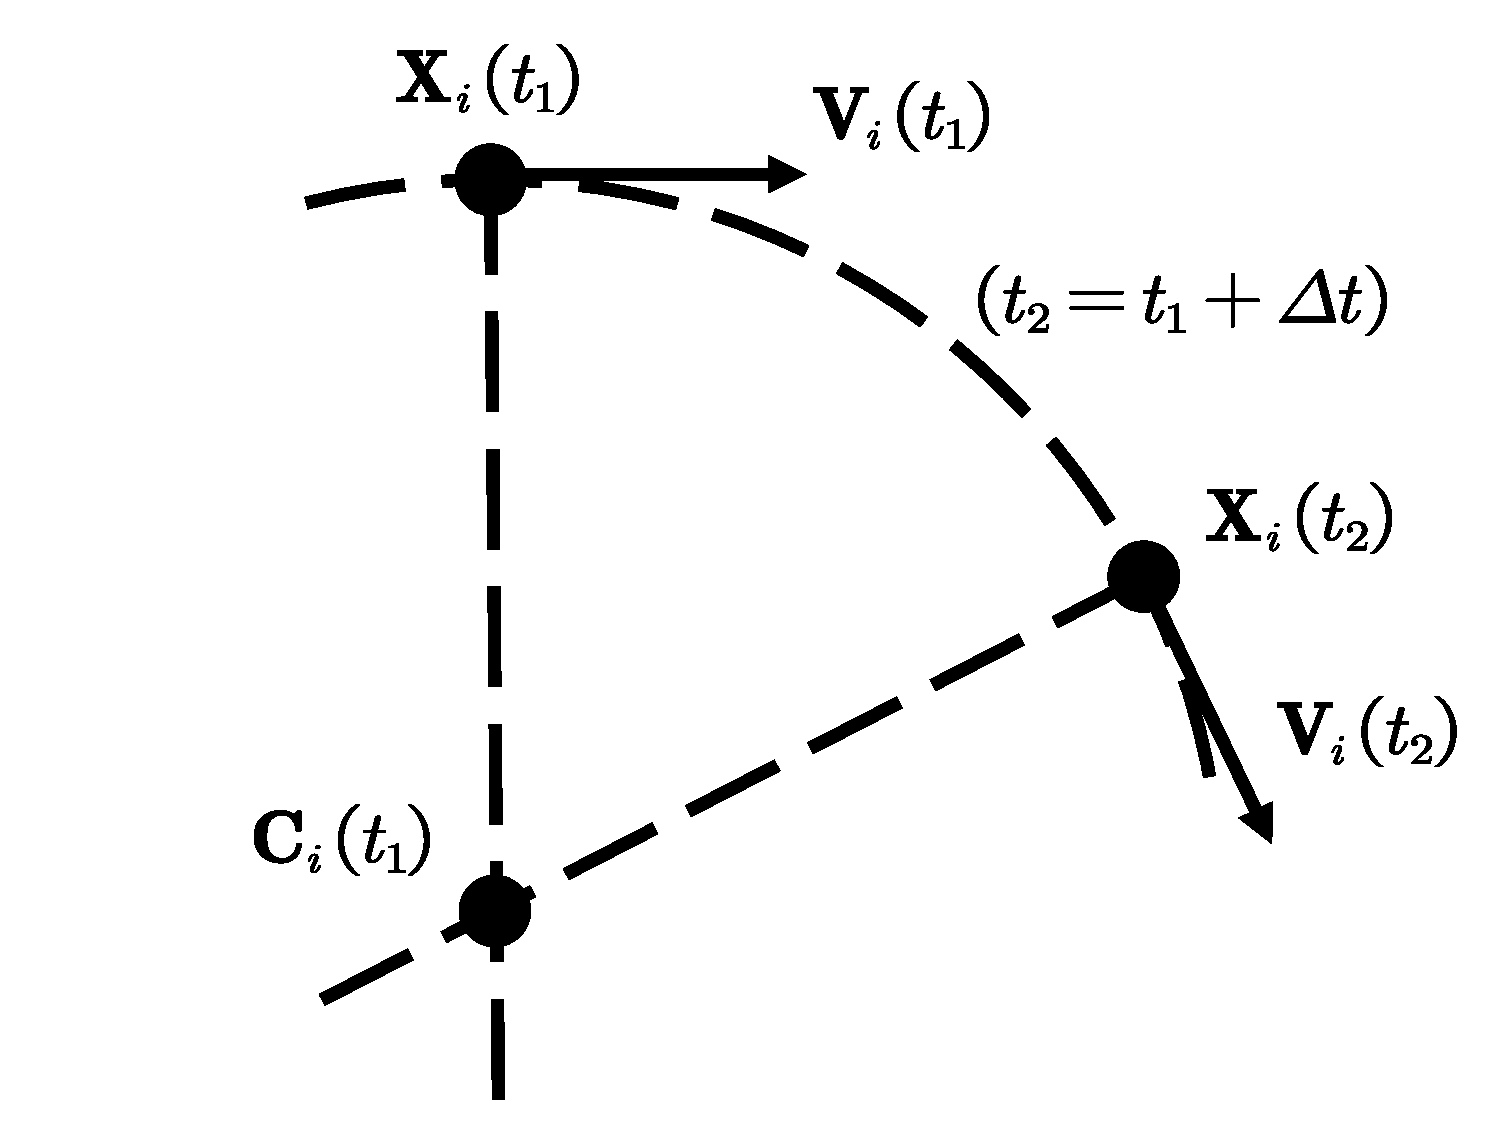
\includegraphics[width=0.3\textwidth]{./figs/CenterEps.pdf}
	\vspace{-0.2cm}
	\caption{旋转圆心示意图}
	\label{fig:fig232.1}
\end{figure}

如图 \ref{fig:fig232.1} 所示,对于任意振子$i$, 其当前坐标为$\mathbf{X}_i\left( t_1 \right)$, 速度为$\mathbf{V}_i\left( t_1 \right)$, 下一时刻的坐标为$\mathbf{X}_i\left( t_2 \right)$, 速度为$\mathbf{V}_i\left( t_2 \right)$, 则其旋转中心坐标为两个时刻法向量所在直线的交点, 假设旋转中心坐标为$\mathbf{C}_i\left( t_1 \right)$, 则有

\vspace{-0.5cm}

$$
\begin{cases}
	\mathbf{C}_i\left( t_1 \right) \cdot \mathbf{V}_i\left( t_1 \right) =\mathbf{X}_i\left( t_1 \right) \cdot \mathbf{V}_i\left( t_1 \right) \\
	\mathbf{C}_i\left( t_1 \right) \cdot \mathbf{V}_i\left( t_2 \right) =\mathbf{X}_i\left( t_2 \right) \cdot \mathbf{V}_i\left( t_2 \right) \\
\end{cases}
$$

求解上述方程组,可以得到每个振子的旋转中心坐标,如下图\ref{fig:fig232.2}:% \ref{fig:fig2}.

\begin{figure}[H]
	\centering
	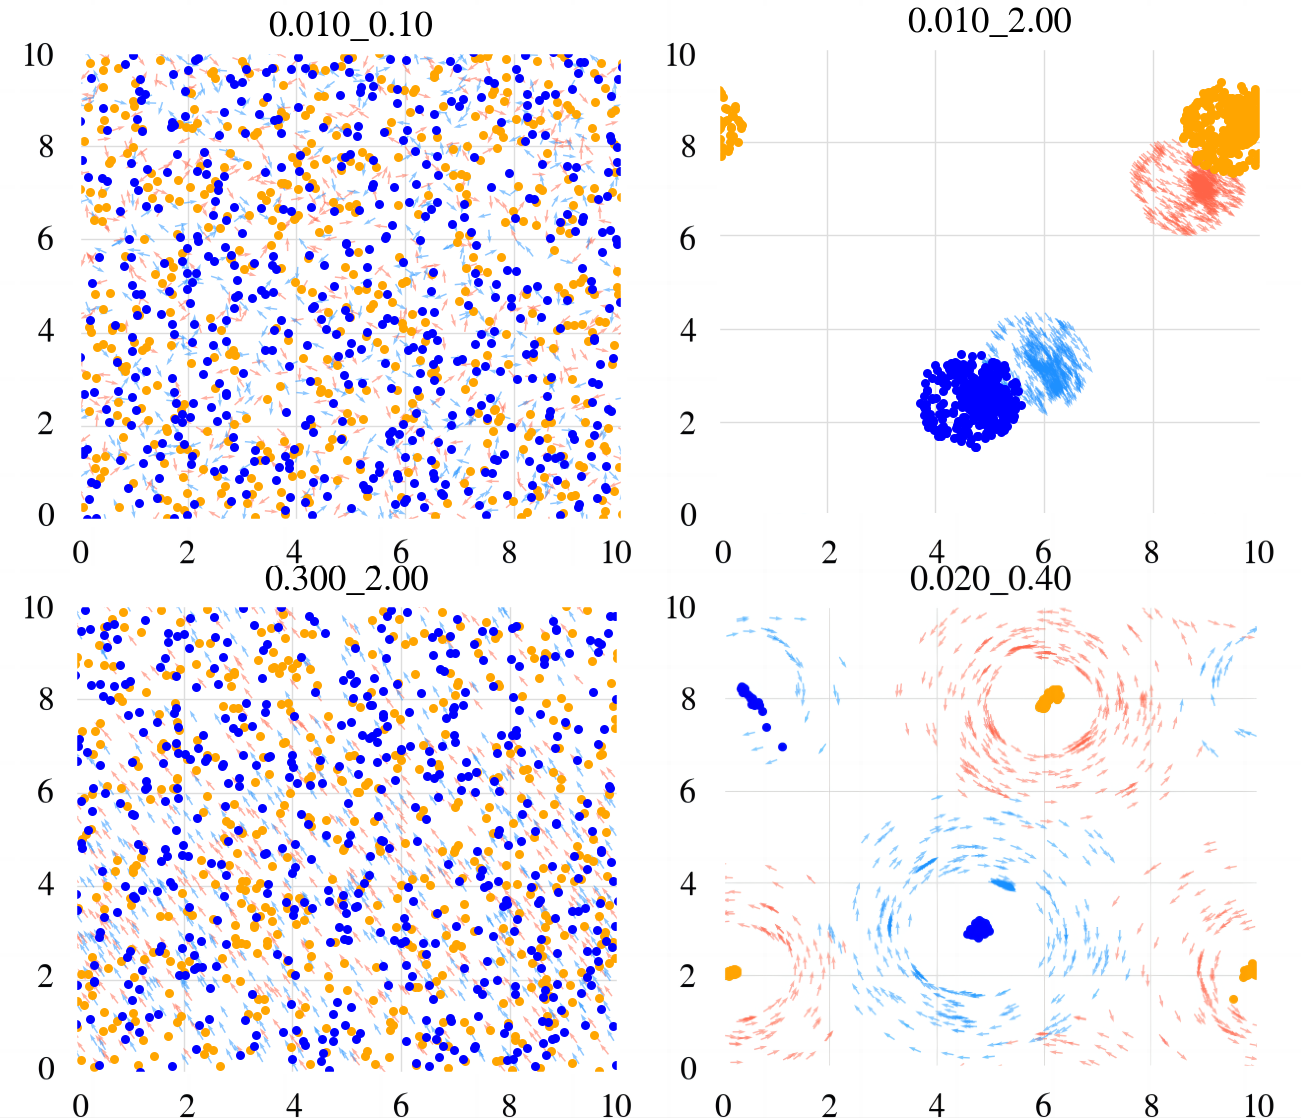
\includegraphics[width=0.7\textwidth]{./figs/centorsBigGraph_sub.png}
	\vspace{-0.2cm}
	\caption{旋转中心求解结果示例}
	\label{fig:fig232.2}
\end{figure}

上图中,带有箭头的半透明色点表示振子,光滑实心色点表示振子的旋转中心,其中,橙色点为正手性振子(半透明红色箭头)的旋转中心,蓝色点为负手性振子(半透明蓝色箭头)的旋转中心. 从图中可以看出,形成清晰的环态后,环上振子的旋转中心较为集中,说明同一环上振子的运动规律较为接近,且近似圆周运动.

\newpage
\noindent\textbf{旋转中心空间分布}

考虑到振子在二维平面上运动,因此该序参量分为$x$坐标和$y$坐标两个分量,将各振子旋转中心坐标以散点图形式分别绘制得到图下图像:

\begin{figure}[H]
	\centering
	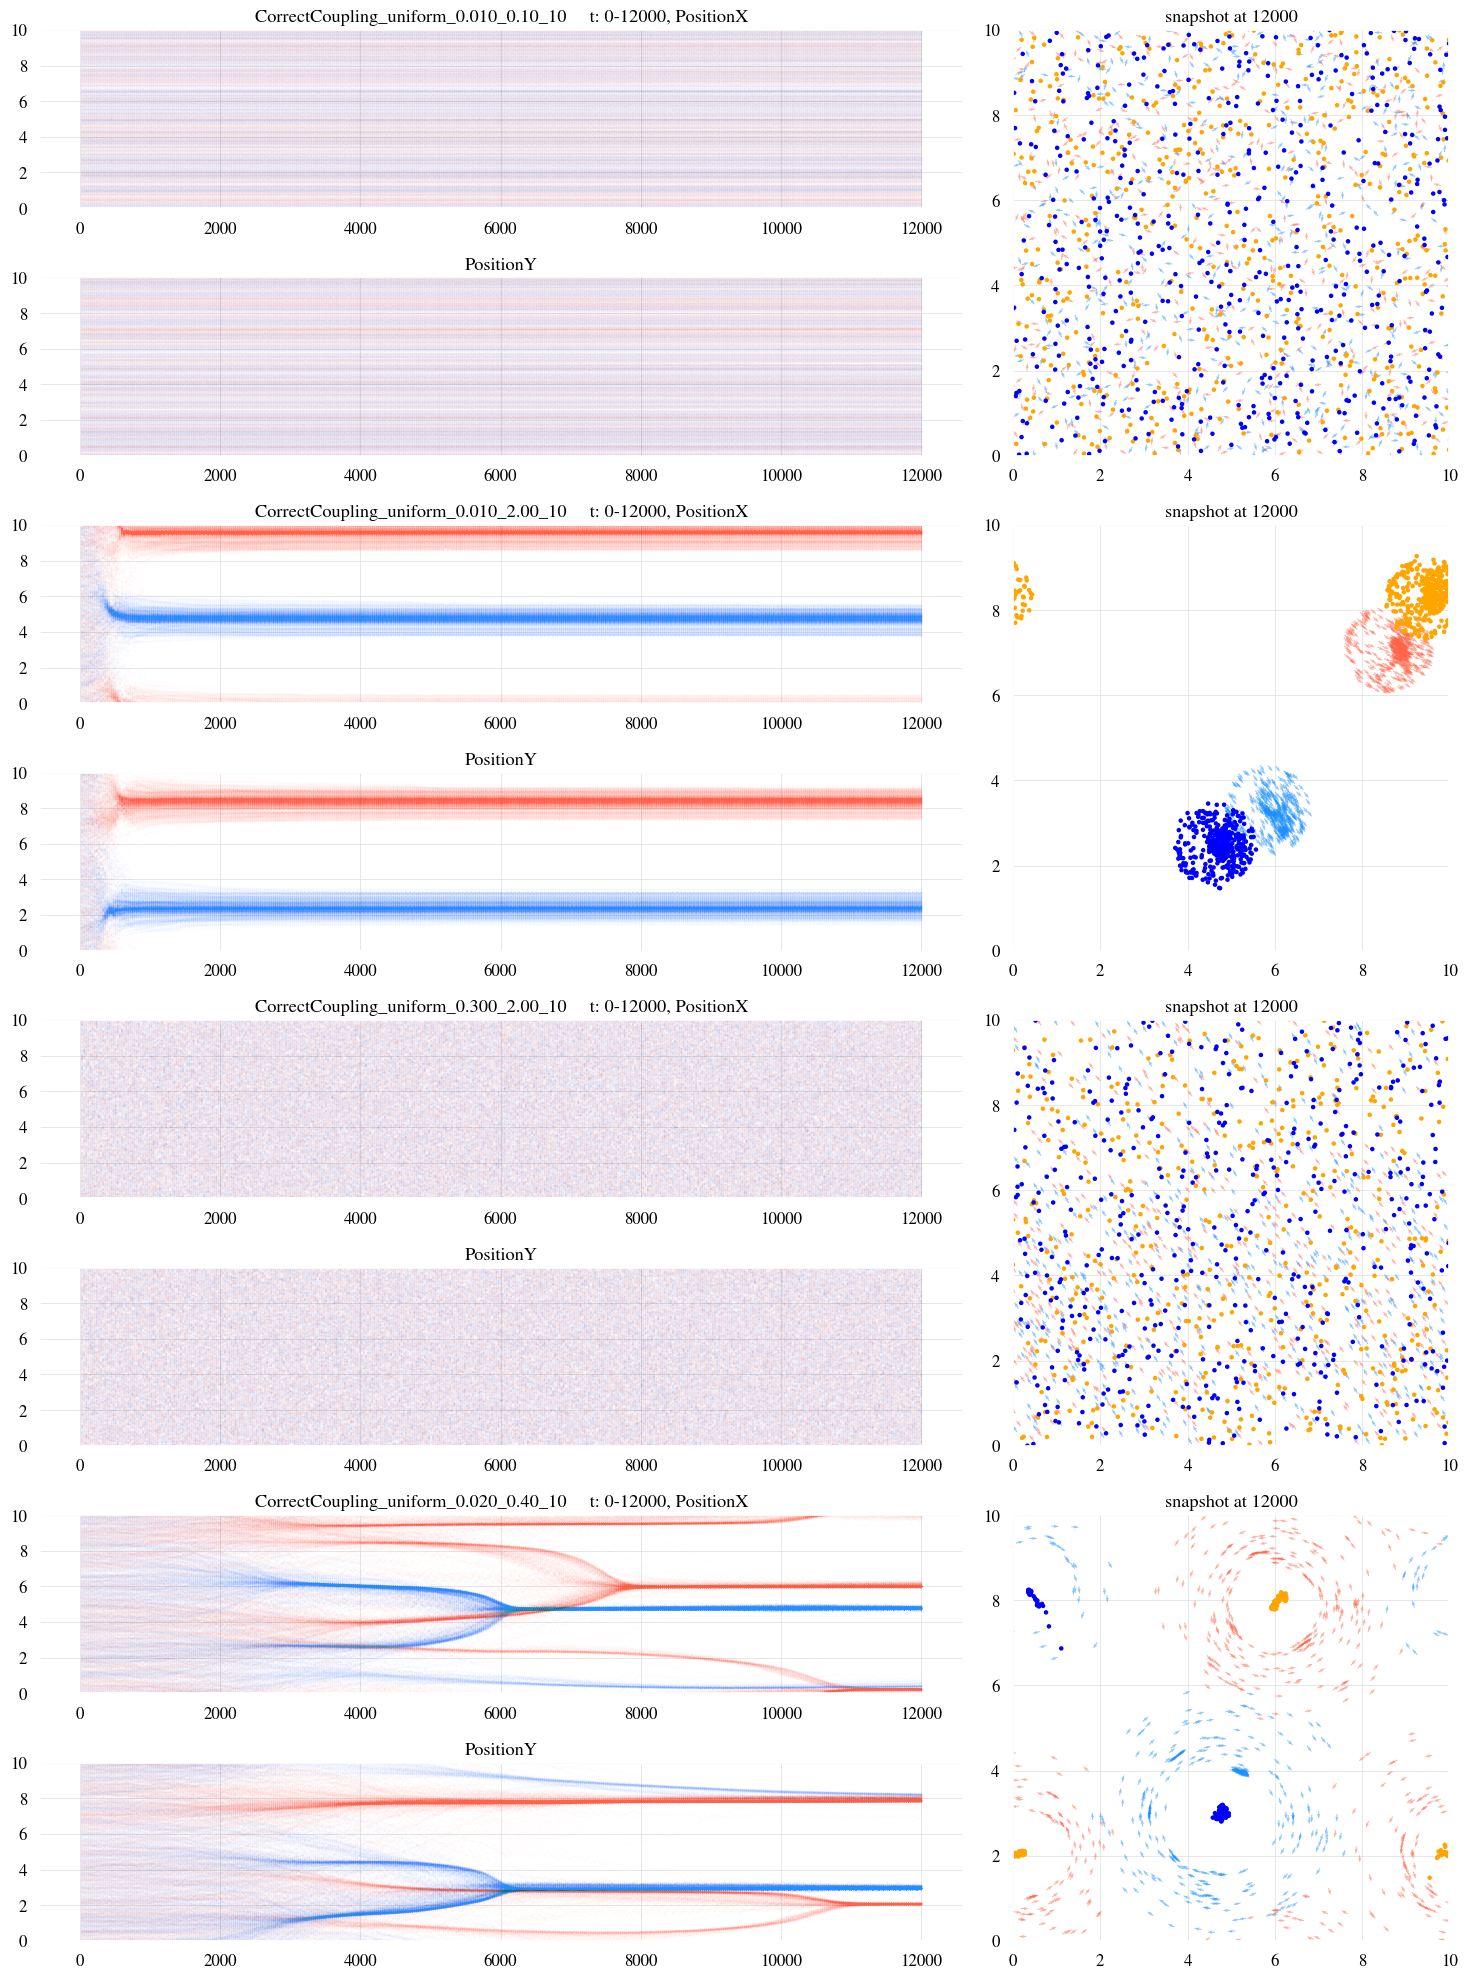
\includegraphics[width=0.9\textwidth]{./figs/totalXY.png}
	\caption{旋转中心空间分布}
	\label{fig:fig234t.1}
\end{figure}

\newpage
\section{序参量}
\begin{figure}[H]
	\centering
	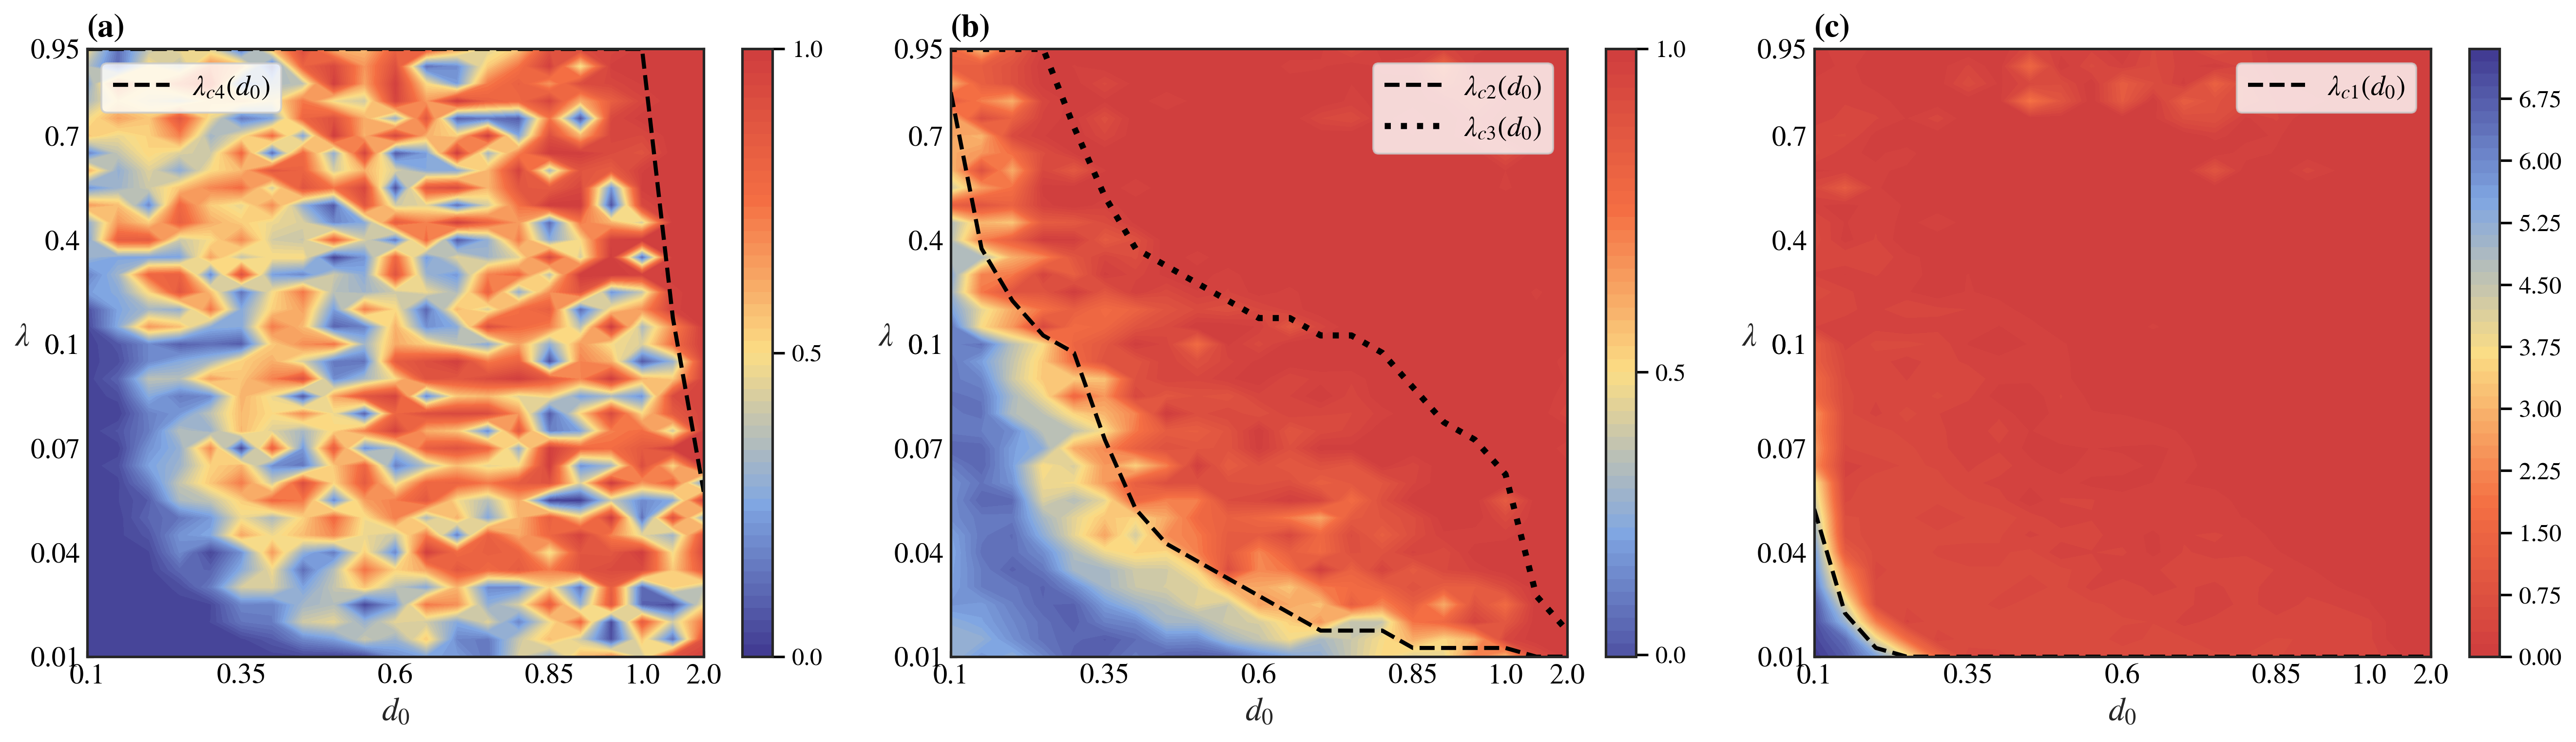
\includegraphics[width=\textwidth]{./figs/orderParam.png}
	\caption{序参量与临界耦合强度}
\end{figure}

上图三张序参量热图分别对应下面三个公式

$$
\mathbf{(a)}: R = \left| \frac{1}{N}\sum_{j=1}^N{e^{i\theta _j}} \right|
$$

$$
\mathbf{(b)}: R_c = \frac{1}{N_{class}}\sum_{k=1}^{N_{class}}{\left| \frac{1}{N_k}\sum_{i\in C_k}{e^{i\theta _i}} \right|}
$$

$$
\mathbf{(c)}: \Delta \Omega =\frac{1}{N_{class}}\sum_{k=1}^{N_{class}}{\left[ \frac{1}{N_{k}^{2}}\sum_{i,j=1}^{N_k}{\left( \left< \dot{\theta}_i \right> -\left< \dot{\theta}_j \right> \right) ^2} \right]}
$$

其中团簇与环的分类由算法\ref{clustering}得到

\newpage
\subsubsection{基于调整耦合距离的聚类算法}\label{clustering}

考虑到振子在形成环态或集群态时,会形成多个环或集群,因此可以对振子进行聚类从而计算各环或群的局部序参量. 由于环在欧氏空间中的分布较为特殊(中空,环与环相邻),因此改为对振子的旋转中心进行聚类. 此外,周期性边界条件会导致振子的旋转中心跨边界,这里采样式\ref{eq:eq1}对旋转中心坐标进行调整.

\begin{algorithm}
	\SetKw{in}{in}
	\SetKwData{Left}{left}\SetKwData{This}{this}\SetKwData{Up}{up}
	\SetKwFunction{Union}{Union}\SetKwFunction{FindCompress}{FindCompress}
	\SetKwInOut{Input}{input}\SetKwInOut{Output}{output}

	\BlankLine
	\KwData{A set $S=\left\{(\bar{x}_i, \bar{y}_i)\right\}$ of particles' circular center coordinates}
	\KwIn{cluster distance $d_{th}$}
	\KwResult{A cluster set $C=\left\{
		\left\{ 1 \right\}
	 \right\}$}
	% \BlankLine
	\emph{$C$ $\leftarrow$ $\left\{(\bar{x}_1, \bar{y}_1)\right\}$}\;
	\For{$i\leftarrow 2$ \KwTo $N$}{\label{forins}
		\For{class set $C_k$ \in $C$}{
			\For{$j$ \in $C_k$}{
				\If(\tcp*[f]{belong to $C_k$}){$\bar{d}_{ij} < d_{th}$}{
					$C_j \leftarrow C_j \cup \left\{i\right\}$\;
					go to line \ref{forins}\;
				}
			}
		}
		$C \leftarrow C \cup \left\{\left\{i\right\}\right\}$; \tcp*[f]{create new class}
	}
	\caption{Clustering algorithm based on adjusted distance}\label{algo_disjdecomp}
\end{algorithm}\DecMargin{1em}

取$d_{th}=1, \lambda=0.02, d_0=0.4, random seed=80$并对模型终态执行算法,可得到如下图\ref{fig:fig233.1}所示的聚类结果. 对比左侧子图与右侧子图,可以发现,算法可以较好地将多个环分开.

\begin{figure}[H]
	\centering
	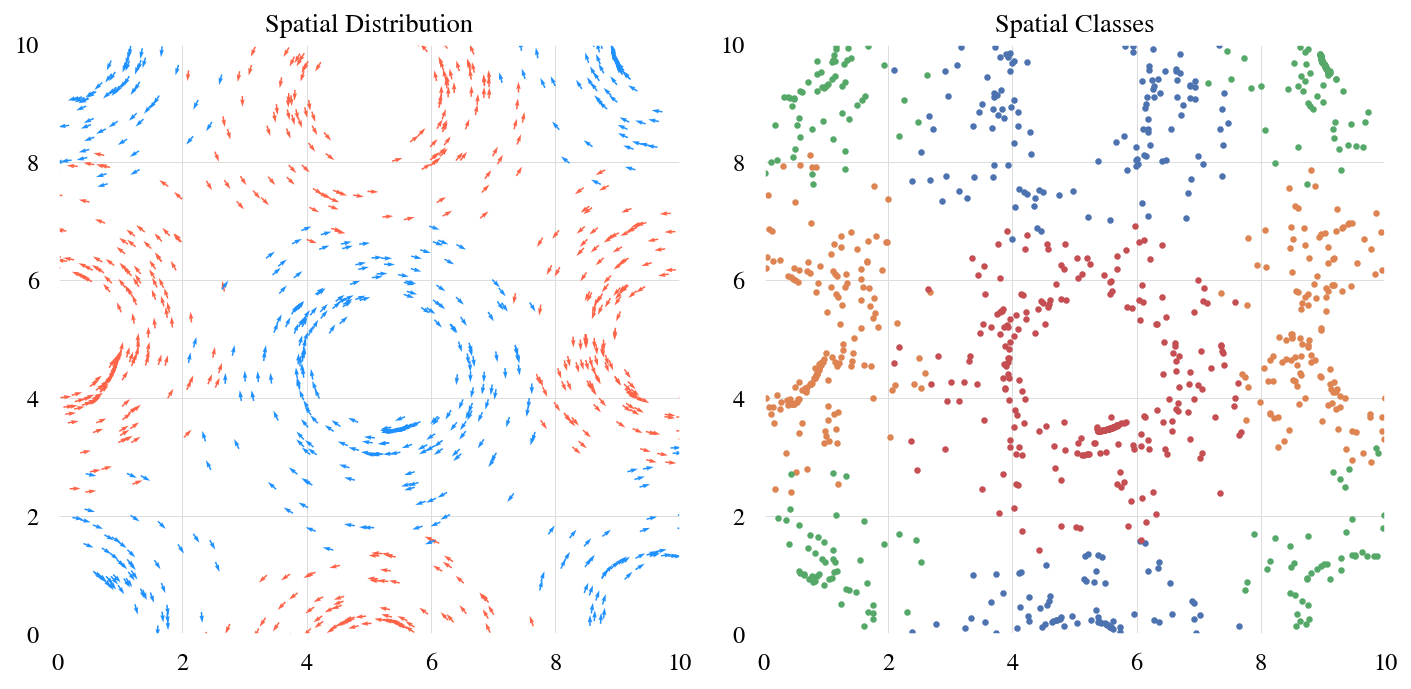
\includegraphics[width=0.9\textwidth]{./figs/ClusteringResult.png}
	\vspace{-0.4cm}
	\caption{聚类结果 ($d_{th}=1, \lambda=0.02, d_0=0.4, random seed=80$)}
	\label{fig:fig233.1}
\end{figure}

\subsubsection{序参量的思考过程}

为了评估截面序参量对相图的刻画能力,这里根据终态的拓扑结构绘制了主观划分的相图,以提供对比,如下图\ref{fig:fig234.1}所示. 从左至右,从上至下,分别为无序态、环态、集群态、瞬时同步态. 图\ref{fig:fig232.2}中的四种状态分别对应图\ref{fig:fig234.1}中的四个区域,对比观察可以发现,环态与集群态在空间上的聚集程度较高,而无序态与瞬时同步态在空间上分布较为均匀,聚集程度低; 此外,集群态与瞬时同步态在相位(速度方向)上的同步程度较高,而环态与无序态较低.

\begin{figure}[H]
	\centering
	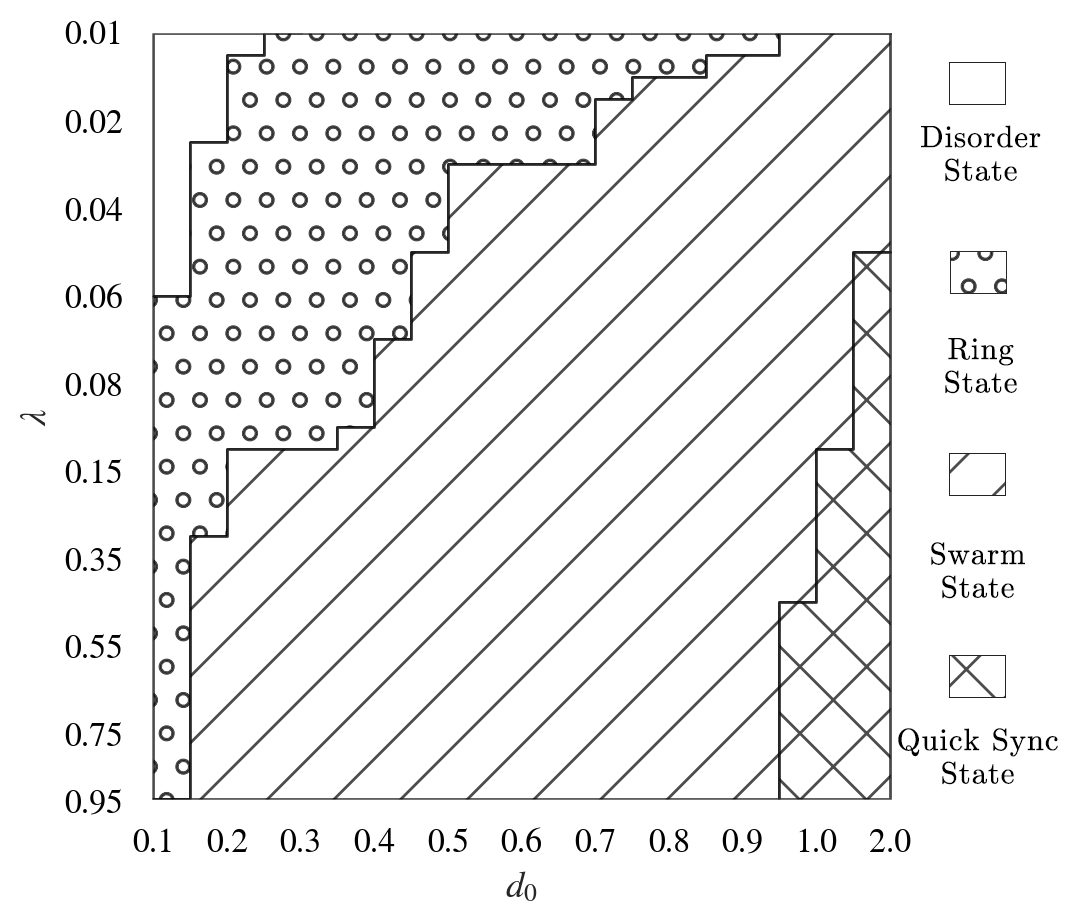
\includegraphics[width=0.5\textwidth]{./figs/subjectiveOp3.png}
	\vspace{-0.5cm}
	\caption{主观划分空间状态图}
	\label{fig:fig234.1}
\end{figure}
\vspace{-0.5cm}

\noindent\textbf{相位(速度方向)同步率}

$$
r e^{i\psi}=\frac{1}{N}\sum_{j=1}^{N}{e^{i\theta _j}}
$$

\begin{figure}[H]
	\centering
	\begin{subfigure}[b]{0.49\textwidth}
		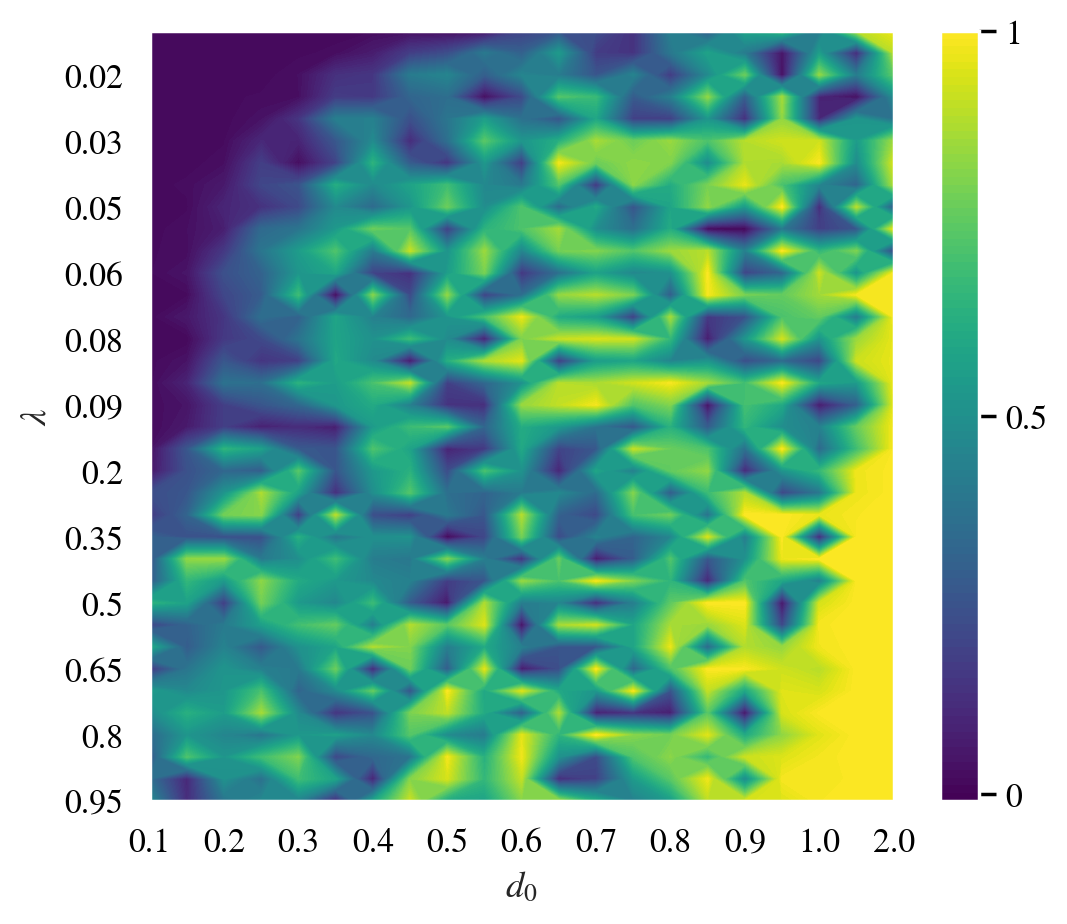
\includegraphics[width=\textwidth]{./figs/phaseSyncOp.png}
		\vspace{-1cm}
		\caption{计算结果}
	\end{subfigure}
	% \hfill
	\begin{subfigure}[b]{0.49\textwidth}
		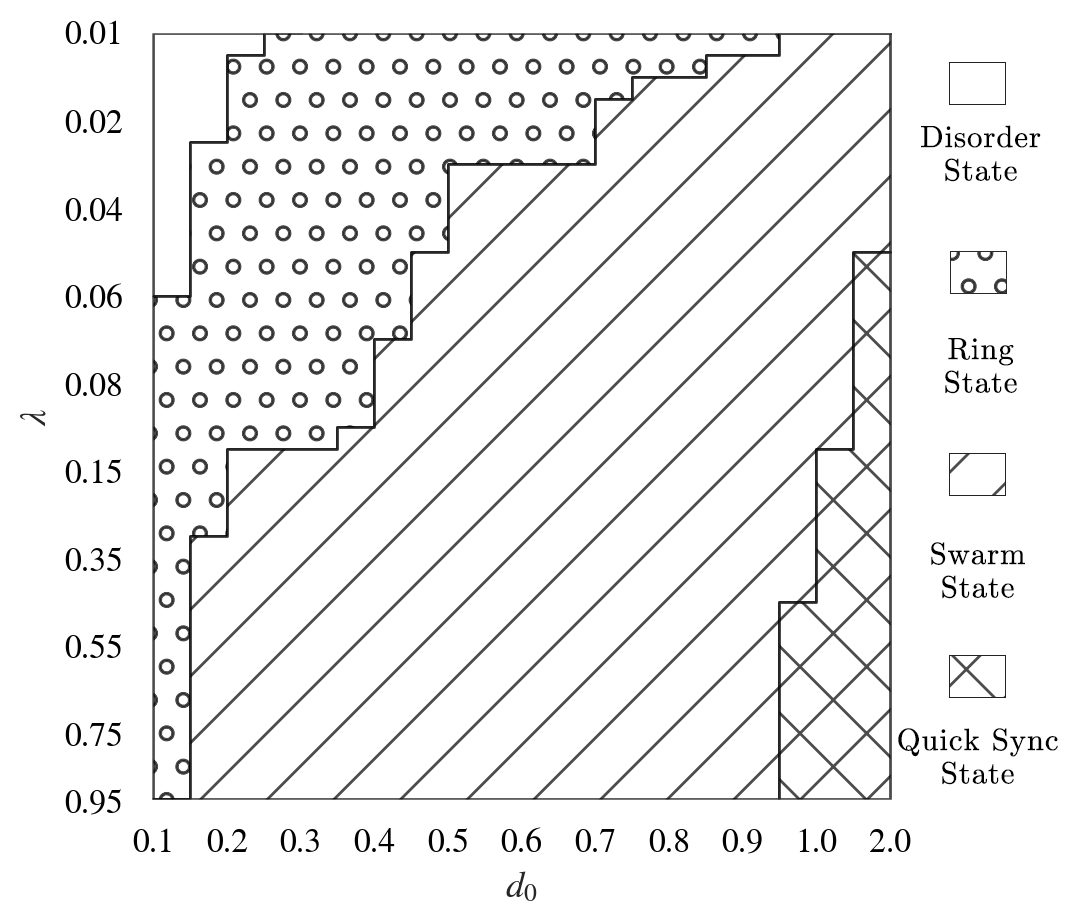
\includegraphics[width=\textwidth]{./figs/subjectiveOp3.png}
		\vspace{-1cm}
		\caption{主观划分空间状态图}
	\end{subfigure}
	\vspace{-0.5cm}
	\caption{相位(速度方向)同步率}
	\label{fig:fig234c.1}
\end{figure}

\vspace{-0.5cm}
该序参量可以将代表全局同步的快速同步态区分. 由于部分集群态存在分裂现象,因此某些集群态的全局相位同步程度较低,导致该序参量过渡不均匀,不易区分环态与集群态. 

\newpage
\noindent\textbf{聚类平均相位同步程度}

这里基于方法\ref{clustering}($d_{th}=0.3$)对振子旋转中心进行聚类,然后计算每一类(振子数不足5个的分类剔除)中振子的相位同步程度,最后取所有类的相位同步程度的算数平均,即

$$\frac{1}{N_{class}}\sum_{k=1}^{N_{class}}\left|\cfrac{1}{N_{k}}\sum_{i\in C_{k}}e^{i\theta_i}\right|$$

\vspace{-0.5cm}
\begin{figure}[H]
	\centering
	\begin{subfigure}[b]{0.49\textwidth}
		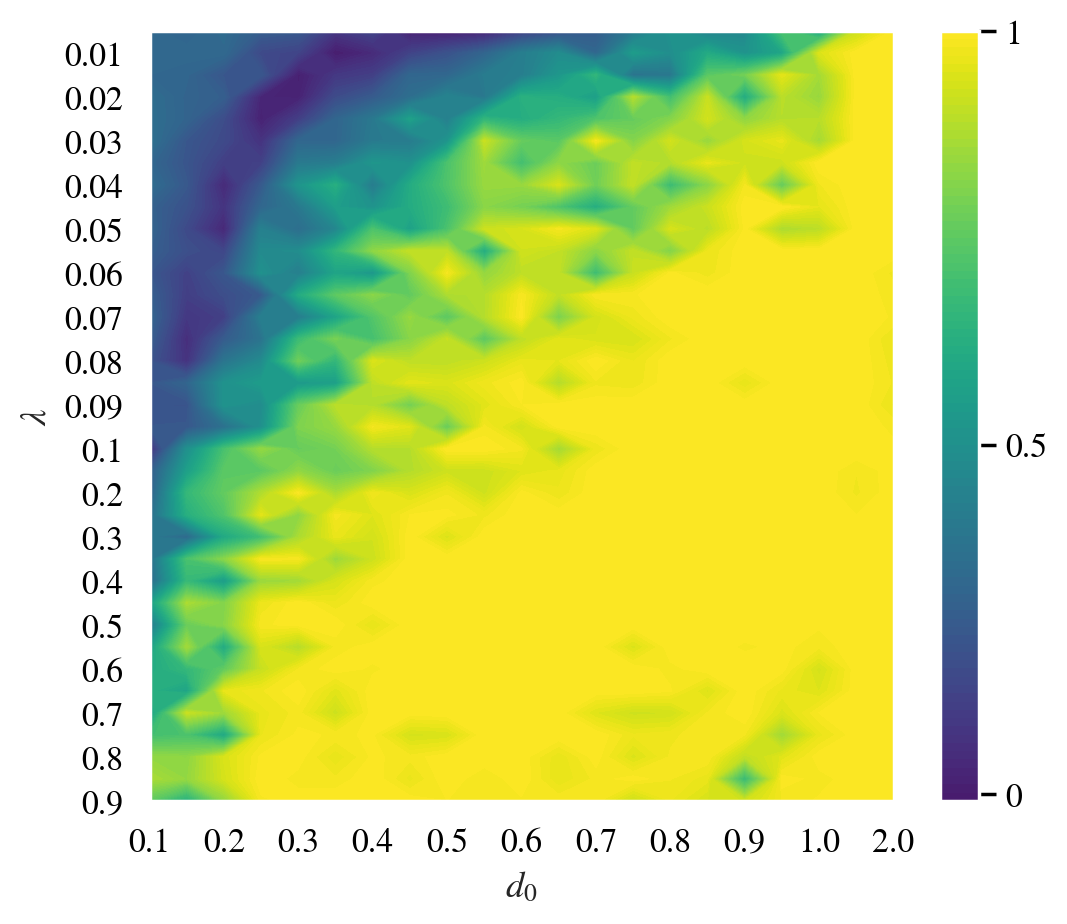
\includegraphics[width=\textwidth]{./figs/clusteringPhaseSync.png}
		\vspace{-1cm}
		\caption{计算结果}
	\end{subfigure}
	% \hfill
	\begin{subfigure}[b]{0.49\textwidth}
		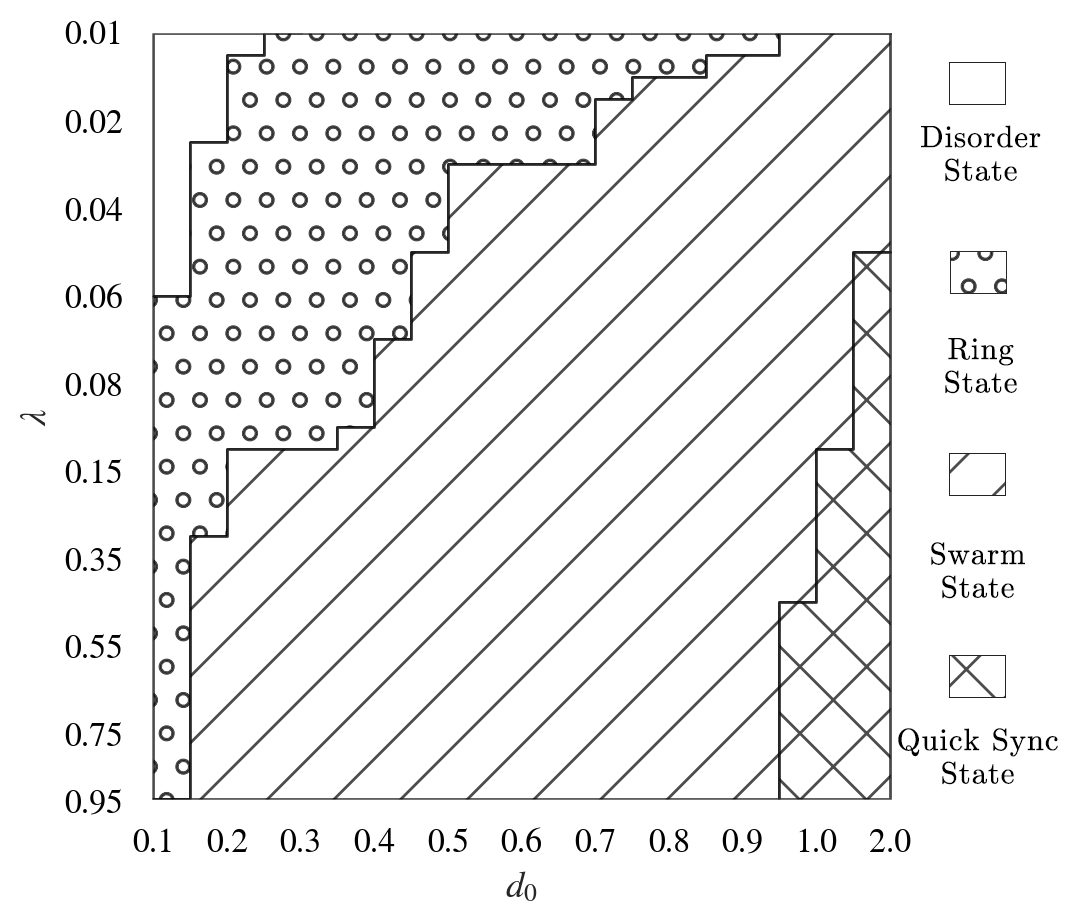
\includegraphics[width=\textwidth]{./figs/subjectiveOp3.png}
		\vspace{-1cm}
		\caption{主观划分空间状态图}
	\end{subfigure}
	\vspace{-0.5cm}
	\caption{聚类平均相位同步程度}
	\label{fig:fig234c.5}
\end{figure}

\vspace{-0.5cm}
对比图\ref{fig:fig234c.1}可以发现,图\ref{fig:fig234c.5}能够更好地刻画环态与集群态的相位同步程度. 

\noindent\textbf{全局平均频率差}

集群行为的讨论既要分析各种不同的空间集群态,也应研究对同步的影响. 除了计算系统序参量以外, 还需要计算振子之间的锁相.

定义平均频率差
$$
\begin{aligned}
	\Delta \Omega _1&=\overline{\left( \left< \dot{\theta}_i \right> -\bar{\Omega} \right) ^2}\\
	\Delta \Omega _2&=\frac{1}{N^2}\sum_{i,j=1}^N{\left( \left< \dot{\theta}_i \right> -\left< \dot{\theta}_j \right> \right) ^2}\\
\end{aligned}
$$

其中,$\left< \cdot \right>$为长时平均,$\overline{\,\,\cdot \,\,}$为系统平均. $\bar{A}=\frac{1}{N^2}\sum\nolimits_i^{}{A_i}$, $\left< A \right> =\lim_{T\rightarrow \infty} \frac{1}{T}\int_{t_0}^{t_0+T}{A\left( t \right) dt}$

这里取$t_0=500$ (50000次迭代, $\mathrm{d}t=0.01$), $T=100$ (10000次迭代, $shotsnaps=5$, 2000个样本点)进行计算.

\begin{figure}[H]
	\centering
	\begin{subfigure}[b]{0.49\textwidth}
		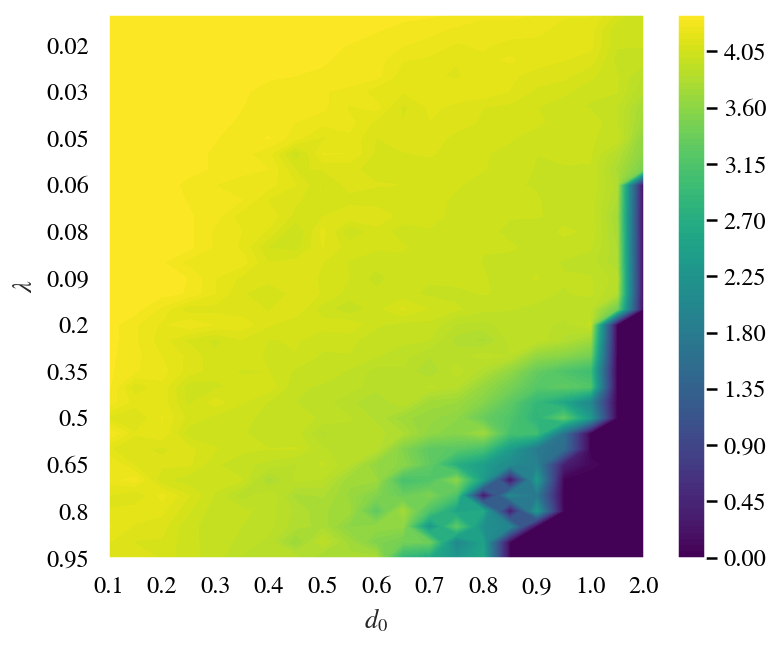
\includegraphics[width=\textwidth]{./figs/deltaOmega1.png}
		\vspace{-1cm}
		\caption{$\Delta \Omega _1$}
	\end{subfigure}
	% \hfill
	\begin{subfigure}[b]{0.49\textwidth}
		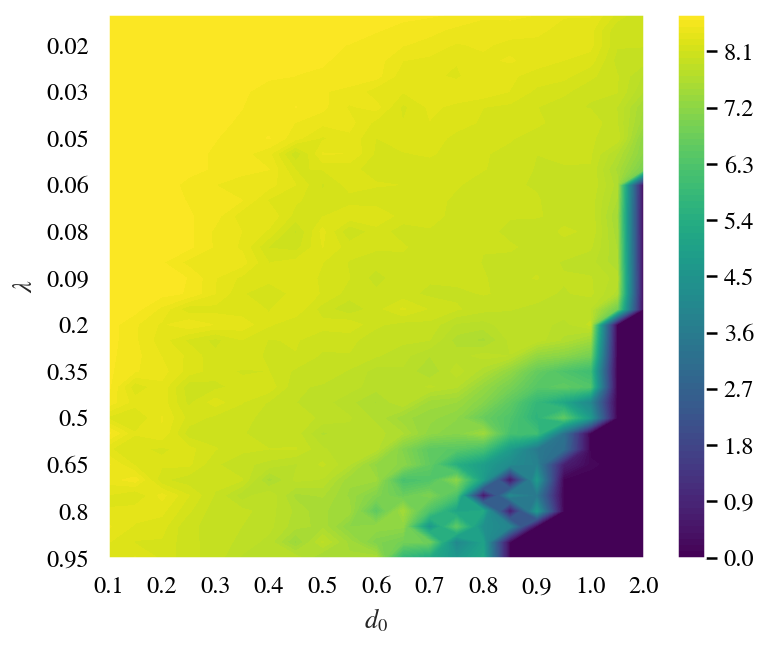
\includegraphics[width=\textwidth]{./figs/deltaOmega2.png}
		\vspace{-1cm}
		\caption{$\Delta \Omega _2$}
	\end{subfigure}
	\vspace{-0.5cm}
	\caption{全局平均频率差}
	\label{fig:fig2.5.global}
\end{figure}

观察图\ref{fig:fig2.5.global}可以发现,$\Delta \Omega _1$与$\Delta \Omega _2$的取值分布基本一致,并且都在瞬时同步态与集群态之间有明显的差异. 处于瞬时同步态或单集群的集群态时,系统发生整体锁相,$\Delta\Omega_1$与$\Delta\Omega_2$趋于0. 考虑到集群态在各个集群内部的同步程度较高,因此下面对集群的平均频率差进行讨论.

\noindent\textbf{聚类平均频率差}

除了对全局平均频率差的讨论,还可以对各个集群的平均频率差进行讨论. 这里对集群的定义采用方法\ref{clustering}($d_{th}=0.3$)进行聚类,然后计算每一类(振子数不足5个的分类剔除)中振子的平均频率差,最后取所有类的平均频率差的算数平均.

$$
\begin{array}{l}
	\Delta \Omega _{1}^{*}=\frac{1}{N_{class}}\sum_{k=1}^{N_{class}}{\overline{\left( \left< \dot{\theta}_i \right> -\bar{\Omega} \right) ^2}}\\
	\Delta \Omega _{2}^{*}=\frac{1}{N_{class}}\sum_{k=1}^{N_{class}}{\left[ \frac{1}{N_{k}^{2}}\sum_{i,j=1}^{N_k}{\left( \left< \dot{\theta}_i \right> -\left< \dot{\theta}_j \right> \right) ^2} \right]}\\
\end{array}
$$

其中,$N_{class}$为集群数,$N_k$为第$k$个集群的振子数. $\overline{\,\,\cdot \,\,}$为集群内平均, 即$\bar{x}=\frac{1}{N_k}\sum_{i\in C_k}{x_i}$

\begin{figure}[H]
	\centering
	\begin{subfigure}[b]{0.49\textwidth}
		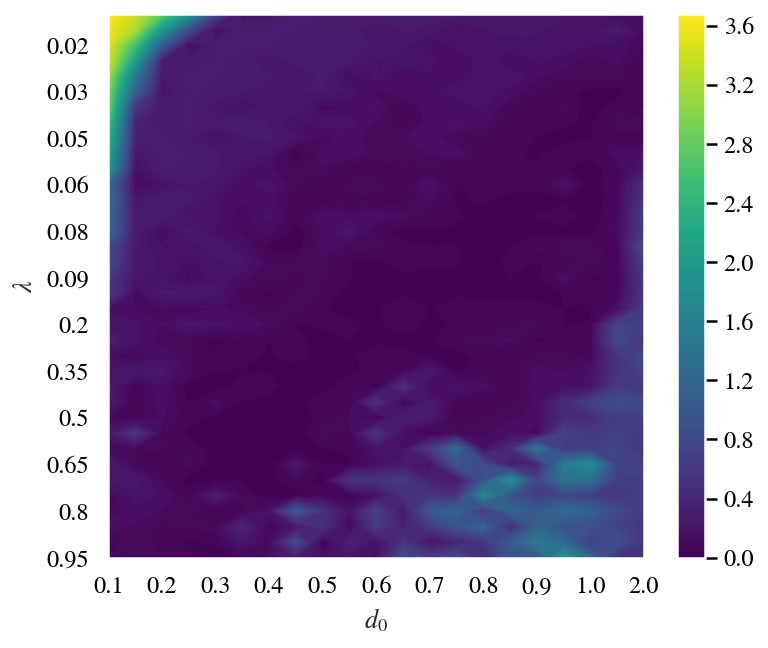
\includegraphics[width=\textwidth]{./figs/clusterDeltaOmega1.png}
		\vspace{-1cm}
		\caption{$\Delta \Omega _{1}^{*}$}
	\end{subfigure}
	% \hfill
	\begin{subfigure}[b]{0.49\textwidth}
		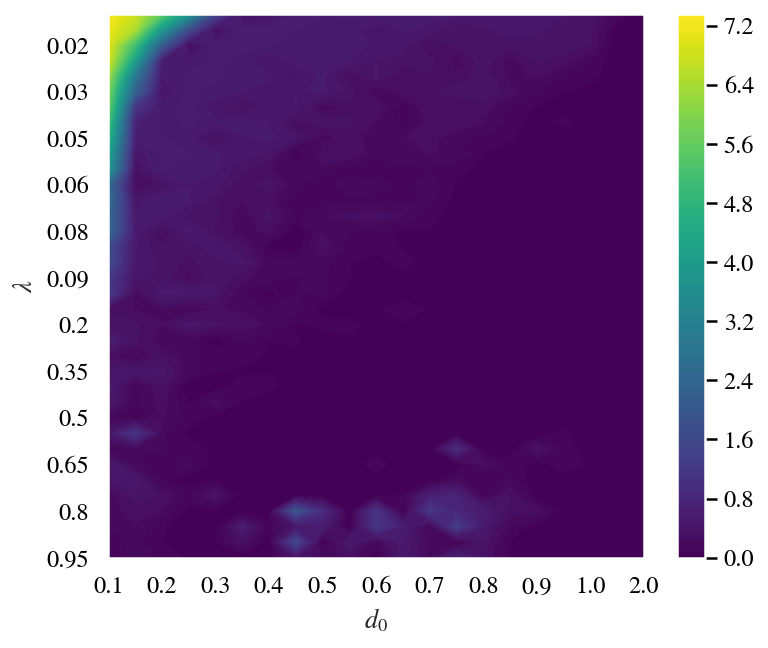
\includegraphics[width=\textwidth]{./figs/clusterDeltaOmega2.png}
		\vspace{-1cm}
		\caption{$\Delta \Omega _{2}^{*}$}
	\end{subfigure}
	\vspace{-0.5cm}
	\caption{聚类平均频率差}
	\label{fig:fig2.5.cluster}
\end{figure}



\newpage
\section{理论分析}
\subsection{单个振子的运动问题(无相互作用)}

$$
\begin{cases}
	\begin{array}{c}
	\Delta x\left( t \right) =v\cos \theta \Delta t\\
	\Delta y\left( t \right) =v\sin \theta \Delta t\\
\end{array}\rightarrow \begin{array}{c}
	\dot{x}=v\cos \theta\\
	\dot{y}=v\sin \theta\\
\end{array}\\
	\dot{\theta}_i=\omega _i\rightarrow \theta _i\left( t \right) =\omega _it\\
	v=\sqrt{\dot{x}_{i}^{2}+\dot{y}_{i}^{2}}=v\left( constant \right)\\
\end{cases}
$$

\textbf{无耦合情况下振子转动半径的求解}

\begin{equation}
    \begin{cases}\label{eq:circle}
        x_i\left( t \right) =x_i\left( 0 \right) +\frac{v}{\omega _i}\sin \omega _it\\
        y_i\left( t \right) =y_i\left( 0 \right) -\frac{v}{\omega _i}\cos \omega _it\\
    \end{cases}
\end{equation}
$$
\Rightarrow \left( x_i-x_{i}^{0} \right) ^2+\left( y_i-y_{i}^{0} \right) ^2=\left( \frac{v}{\omega _i} \right) ^2
$$

每个振子的运动轨迹是一个圆,圆心为 $\left( x_i^0,y_i^0 \right)$,半径为 $\frac{v}{\omega _i}$

\begin{figure}[H]
	\centering
	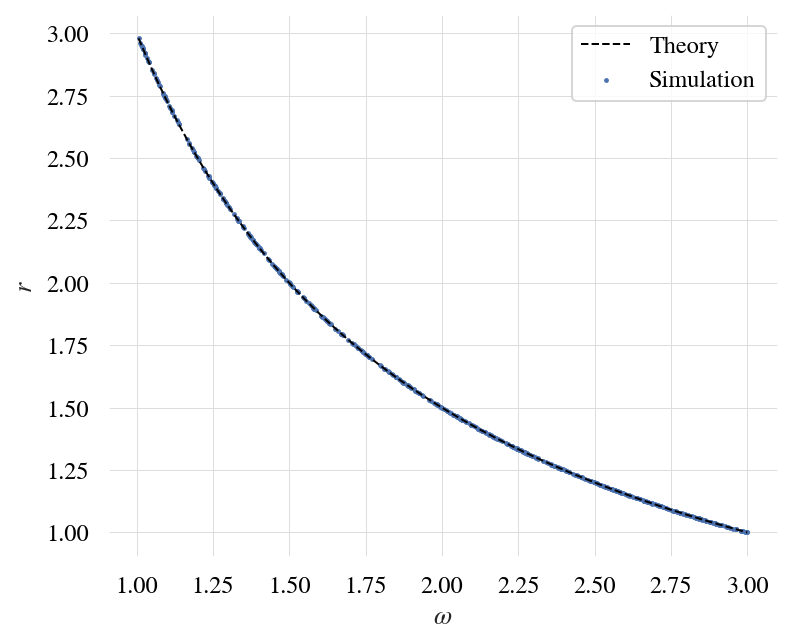
\includegraphics[width=0.5\textwidth]{./figs/noCouplingRadius.png}
	\caption{解析解与数值模拟结果 ($\lambda=0, d_0=0, random seed=10$, Single Chirality)}
	\label{fig:fig21.1}
\end{figure}

\begin{figure}[H]
	\centering
	\begin{subfigure}[b]{0.49\textwidth}
		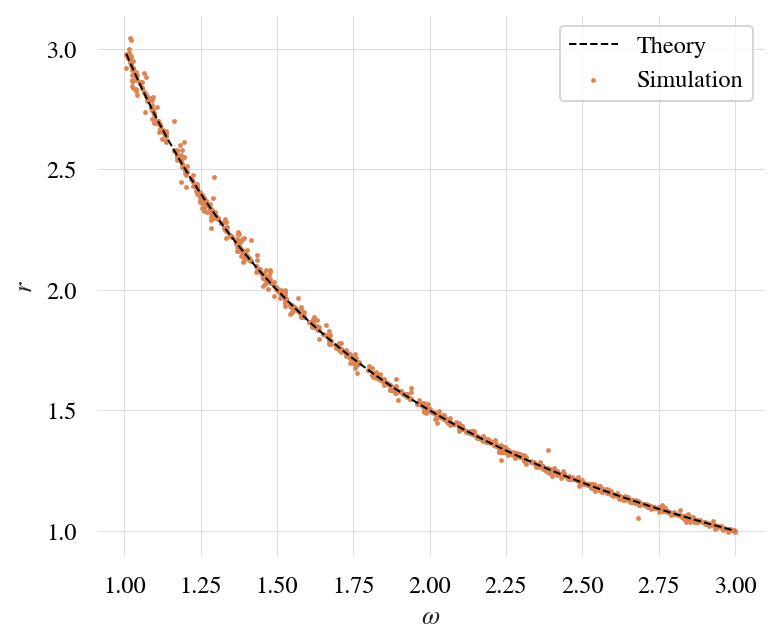
\includegraphics[width=\textwidth]{./figs/DisorderStateRadius.png}
		\vspace{-1cm}
		\caption{无序态 ($\lambda=0.01:0.03$)}
	\end{subfigure}
	% \hfill
	\begin{subfigure}[b]{0.49\textwidth}
		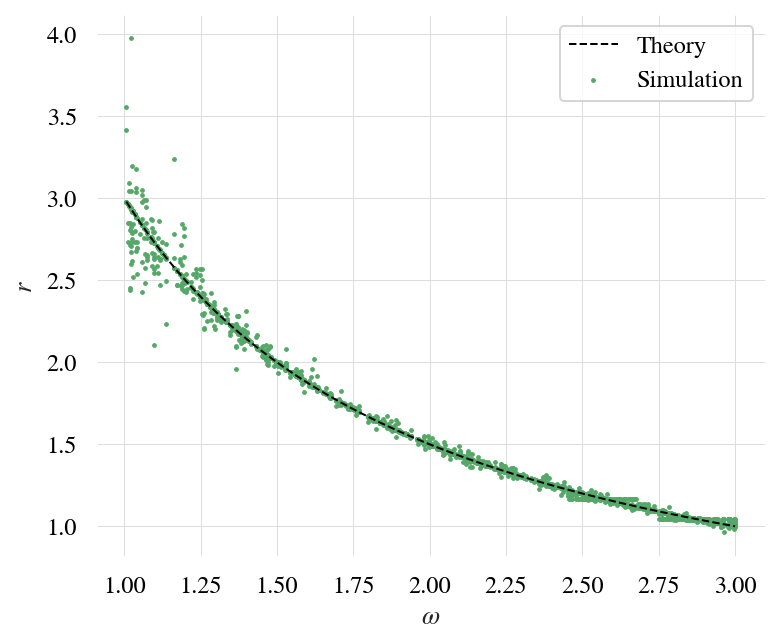
\includegraphics[width=\textwidth]{./figs/RingStateRadios.png}
		\vspace{-1cm}
		\caption{环态 ($\lambda=0.04:0.1$)}
	\end{subfigure}
	\vspace{-0.5cm}
	\caption{无序态、环态解析解与数值模拟结果 ($d_0=0.1, random seed=10$ Single Chirality)}
	\label{fig:fig21.2}
\end{figure}

\begin{figure}[H]
	\centering
	\begin{subfigure}[b]{0.49\textwidth}
		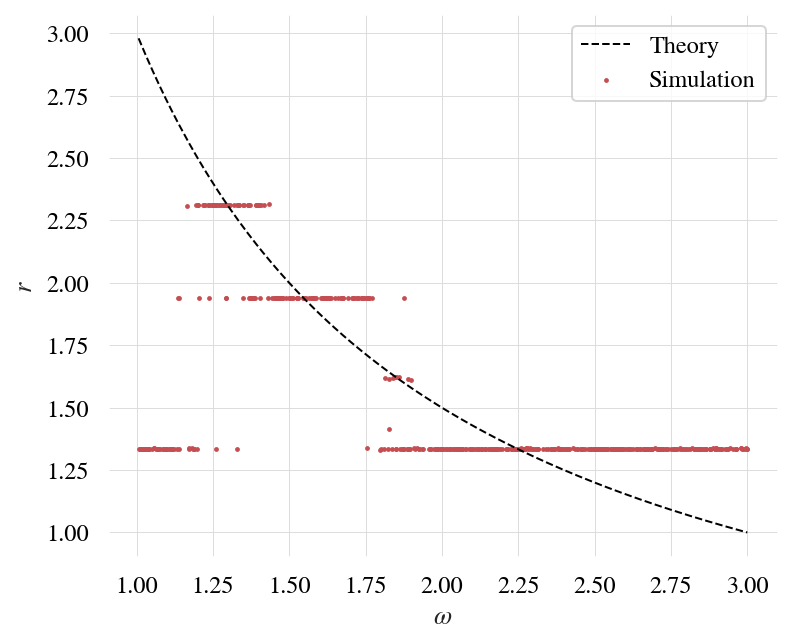
\includegraphics[width=\textwidth]{./figs/SwarmStateRadius.png}
		\vspace{-1cm}
		\caption{$\omega_i = \left| \mathbf{X}_i - \mathbf{C}_i\right|$}
	\end{subfigure}
	% \hfill
	\begin{subfigure}[b]{0.49\textwidth}
		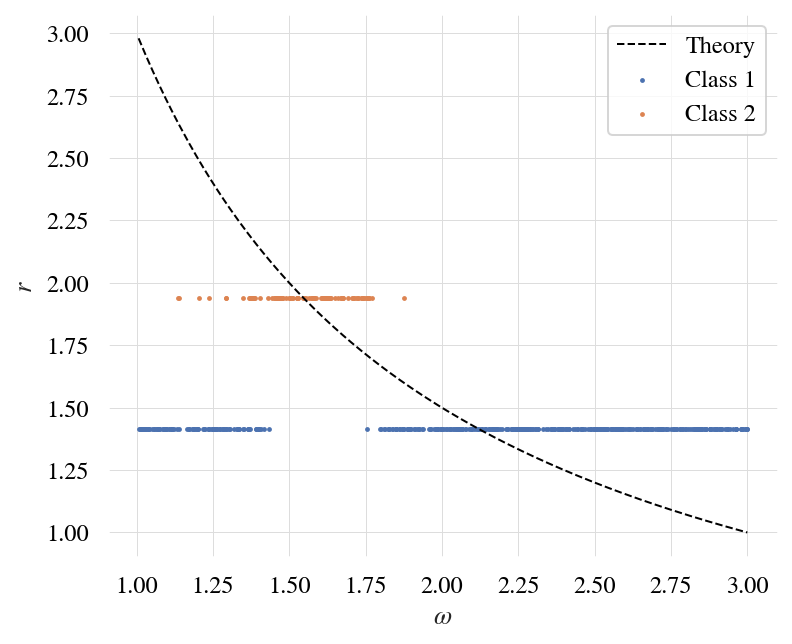
\includegraphics[width=\textwidth]{./figs/classMeanOmegaRadius.png}
		\vspace{-1cm}
		\caption{$\hat{\omega}_k = (\sum\nolimits_{i \in C_k}^N{\omega _i}) / N$}
	\end{subfigure}
	\vspace{-0.5cm}
	\caption{集群态旋转半径的近似 ($\lambda=0.1, d_0=0.3, random seed=10$, Single Chirality)}
	\label{fig:fig21.4}
\end{figure}

\subsection{集群态相速度的推导}\label{swarmPointTheta}

考虑到集群态振子的运动轨迹是一个圆,即对于任意的振子$i$,其运动轨迹为

$$
\left( x_i-x_{i}^{0} \right) ^2+\left( y_i-y_{i}^{0} \right) ^2=\left( \frac{v}{\dot{\theta}_i} \right) ^2
$$

其中,$\left( x_{i}^{0},y_{i}^{0} \right)$为振子$i$的初始坐标,$v$为振子的运动的线速度,$\dot{\theta}_i$为振子$i$的相速度,即振子运动的角速度. 由于集群态振子运动轨迹的半径相同,因此对于任意的振子$i$与振子$j$,有

$$
\left( \frac{v}{C} \right) ^2=\left( \frac{v}{\dot{\theta}_i} \right) ^2,i=1,2,\cdots ,N
$$

其中$C$为常数,即所有振子具有相同的相速度. 又由于

$$
\dot{\theta}_i=\omega _i+\lambda \sum_{j=1}^N{A_{ij}\sin \left( \theta _j-\theta _i \right)}
$$

求和后得到
\vspace{-0.5cm}

$$
\begin{aligned}
	NC&=\sum_{i=1}^N{\left( \omega _i+\lambda \sum_{j=1}^N{A_{ij}\sin \left( \theta _j-\theta _i \right)} \right)}\\
	C&=\frac{1}{N}\sum_{i=1}^N{\omega _i}+\frac{\lambda}{N}\sum_{i=1}^N{\sum_{j=1}^N{A_{ij}\sin \left( \theta _j-\theta _i \right)}}\\
\end{aligned}
$$

再根据$A_{ij}=A_{ji}$以及$\sin \left( \theta _j-\theta _i \right)=-\sin \left( \theta _i-\theta _j \right)$可得$
A_{ij}\sin \left( \theta _j-\theta _i \right) =-A_{ji}\sin \left( \theta _i-\theta _j \right) 
$

从而有

$$
\sum_{i=1}^N{\sum_{j=1}^N{A_{ij}\sin \left( \theta _j-\theta _i \right)}}=0
$$

因此
\vspace{-0.5cm}

\begin{equation}\label{eq:eq2.2.1}
	C=\frac{1}{N}\sum_{i=1}^N{\omega _i}
\end{equation}

即集群中振子的相速度为集群中所有振子自然频率的算数平均.

\begin{figure}[H]
	\centering
	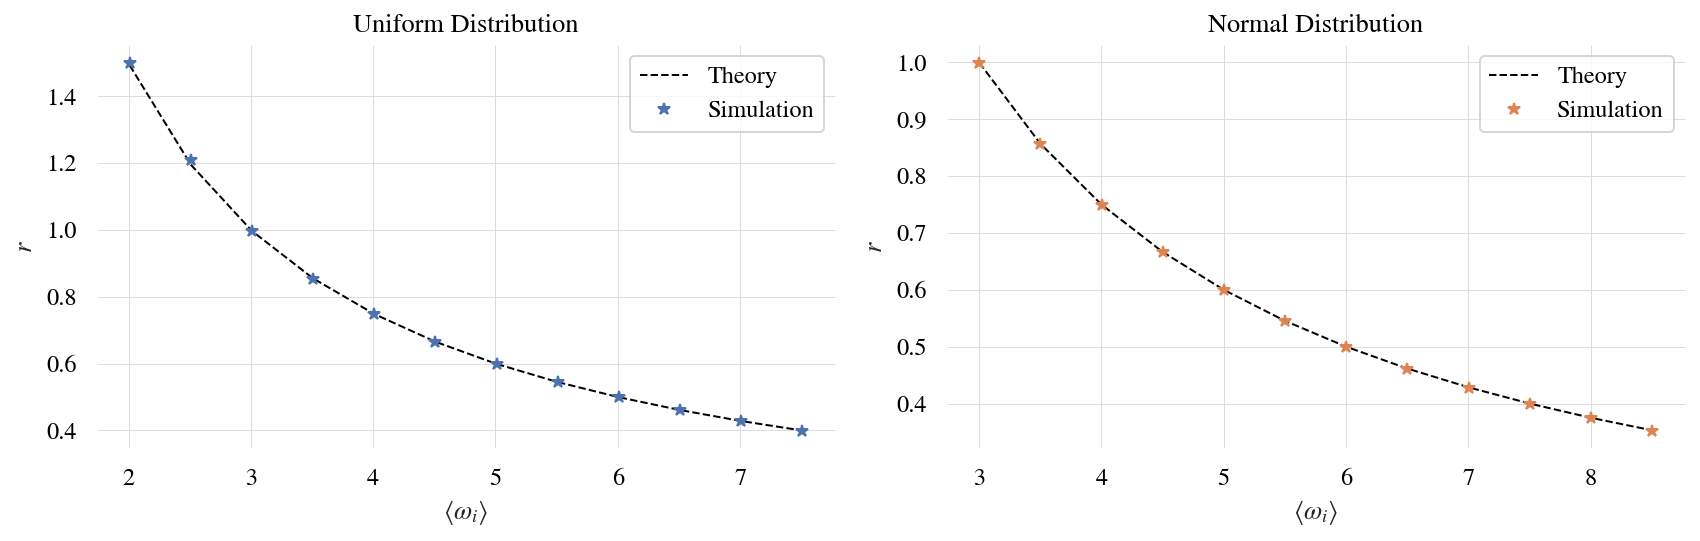
\includegraphics[width=\textwidth]{./figs/swarmRadiusSimu.png}
	\vspace{-1cm}
	\caption{集群态相速度模拟 ($\lambda=0.02, d_0=1, random seed=10$, Single Chirality)}
	\label{fig:fig22}
\end{figure}

\vspace{-0.5cm}

可以看到,在均匀分布与高斯分布的情况下,集群态的相速度都接近于自然频率的算数平均.

\subsection{给定作用半径$d_0$下临界耦合强度$\lambda_c$的求解}

\begin{figure}[H]
    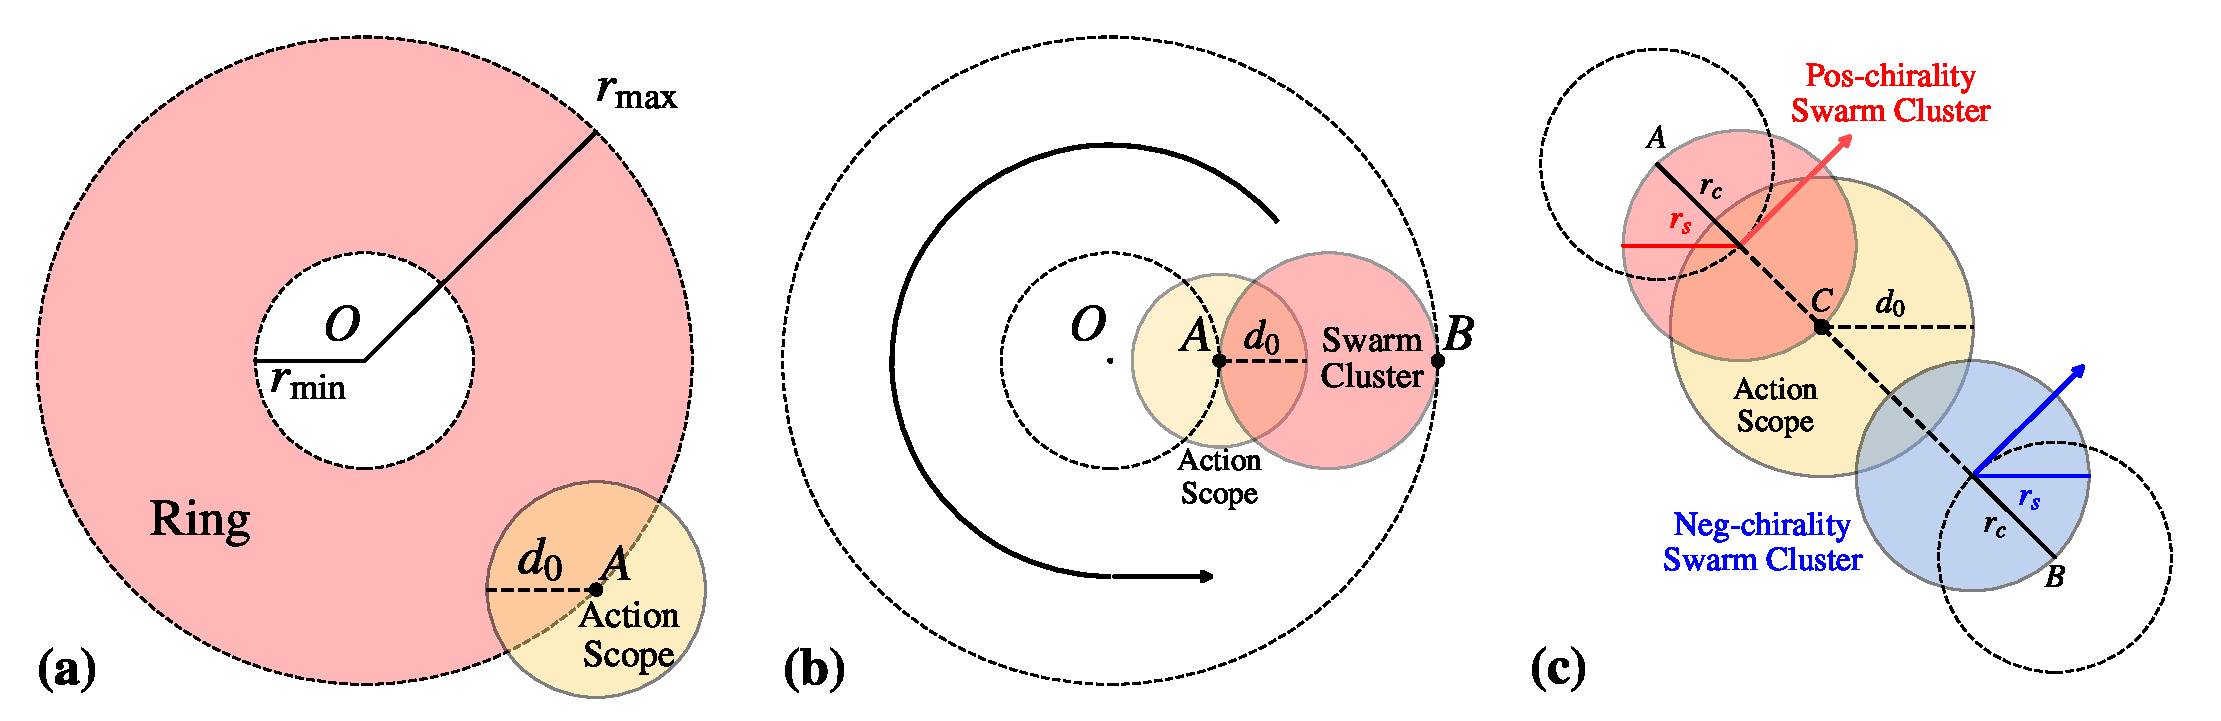
\includegraphics[width=\textwidth]{./figs/analyticalEps.pdf}
    \caption{
        \label{fig:analyticalEps}临界耦合强度求解示意图
    }
\end{figure}

\subsubsection{环态临界耦合强度$\lambda_{c1}$}

我们首先考虑无序态和环态之间的过渡. 这两种状态下的振子都沿着一个圆形的轨迹运动,两者之间的区别是在环状态下的振子是锁相的. 因此,处于无序状态的振子在环上随机分布的概率很小,但没有锁相. 临界耦合强度λc1可以计算为同一环上振子锁相的临界值λ. 我们考虑以下在同一环上的振子的同步动力学:

\begin{equation}\label{eq:eq2}
    \begin{aligned}
        \dot{\theta}_1&=\omega _1+\lambda \sum_{j=2}^{N_c}{A_{1j}\sin \left( \theta _j-\theta _1 \right)}\;,\\
        \dot{\theta}_j&=\omega _j\;,\\
    \end{aligned}
\end{equation}

其中,$N_c$为同一个环上的振子数,$\theta_1$为即将被锁相的振子的相位. 引入$\Delta\omega_j=\omega_j-\omega_1$, 得到

\begin{equation}
    \label{eq:dotDeltaTheta}
    \Delta\dot{\theta}_j=\Delta \omega _j+\lambda \sum_{k=2}^{N_c}{A_{jk}\sin \Delta \theta _k}\;.
\end{equation}

为了实现锁相,环上的每个粒子仅需要与其邻近($\Delta\omega_j$取得最小值)的振子锁相. 在一个环上$\Delta\omega_j$的最小值为$\left| \Delta \omega _j \right|=\left( \omega _{\max}-\omega _{\min} \right) /N_c$. 当$\lambda \sum_{k=2}^{N_c}{A_{jk}} \geqslant \left| \Delta \omega _j \right|$时,方程(\ref{eq:dotDeltaTheta})有不动点解,振子相位锁定. 因此,临界耦合强度$\lambda_{c1}$为:
\begin{equation}
    \lambda _{c1}=\frac{\omega _{\max}-\omega _{\min}}{N_c\sum\nolimits_{j=2}^{N_c}{A_{1j}}}\;,
\end{equation}
其中$\sum\nolimits_{j=2}^{N_c}{A_{1j}}$是环上第1个振子作用范围内的振子数量. 显然,这是关于$d_0$的函数. 我们定义它为
\begin{equation}
    N_1\left( d_0 \right) =N_c\frac{S_1\left( d_0 \right)}{S_R}=\frac{N_cS_1\left( d_0 \right)}{\pi \left( r_{\max}^{2}-r_{\min}^{2} \right)}\;,
\end{equation}
其中$S_1$是第1个振子和环的作用范围的重叠面积,$S_R$是环的面积,$r_{\max}=v/\omega_{\min}$和$r_{\min}=v/\omega_{\max}$分别是环的外半径和内半径. 为了实现环上所有振子的相位锁定,我们需要考虑$N_1\left( d_0\right)$的最小值. 如图(图\ref{fig:analyticalEps}(a))所示,第1个振子位于环的外边缘上的点$A$,黄色圆圈(作用范围)与红色环的重叠面积为$S_1\left( d_0 \right)$. 根据初等几何有
\begin{equation}\label{eq:S1}
    \begin{cases}
        S_1\left( d_0 \right) =d_{0}^{2}\frac{\alpha}{2}+r_{\max}^{2}\frac{\beta}{2}-r_{\max}d_0\sin \frac{\alpha}{2}\\
        \beta =2\mathrm{arc}\cos \left( 1-\frac{d_{0}^{2}}{2r_{\max}^{2}} \right)\\
        \alpha =\pi -\frac{\beta}{2}\\
    \end{cases}\;,
\end{equation}
其中$\alpha$和$\beta$是两个重叠圆心与交点构成的两个扇形的圆心角. 综上所述,我们有
\begin{equation}
    \begin{cases}
        \lambda _{c1}=\frac{\pi \left( r_{\max}^{2}-r_{\min}^{2} \right) \left( \omega _{\max}-\omega _{\min} \right)}{N_{c}^{2}\left( d_{0}^{2}\frac{\alpha}{2}+r_{\max}^{2}\frac{\beta}{2}-r_{\max}d_0\sin \frac{\alpha}{2} \right)}\\
        \beta =2\mathrm{arc}\cos \left( 1-\frac{d_{0}^{2}}{2r_{\max}^{2}} \right)\\
        \alpha =\pi -\frac{\beta}{2}\\
    \end{cases}\;. 
\end{equation}

\subsubsection{集群态临界耦合强度$\lambda_{c2}$}

由于同手性振子的相互作用会导致振子的聚集现象, 因此可以假设在耦合强度与作用半径小于且充分接近临界值的情况下, 全体同手性振子会聚集成环. 假设在耦合强度与作用半径大于临界值且恰巧形成集群的情况下,同手性振子会在保持原转动半径的情况下聚集成群,如图\ref{fig:analyticalEps}(b)所示.

设振子$i$是最后一个即将被同步到集群的振子,其自然频率为$\omega _i$,在以$O$为圆心,$r_{\min}\leqslant r\leqslant r_{\max}$的环带上运动,其余振子$j$恰巧形成集群($j=1,\cdots ,i-1,i+1,\cdots ,N$),即$\dot{\theta}_j=\omega_s$. 由于该集群恰巧形成,此时其中振子仍保留原圆周运动的转动半径,因此集群圆内切环带外边界于点$B$,外切环带内边界于点$A$. 由于集群内的振子数远大于1,且原模型的振子耦合为加性耦合,因此这里忽略振子$i$对集群的作用. 考虑与\ref{eq:eq2}相图的同步动力学, 引入新的变量$\Delta \theta =\theta _i-\theta _j$, $\Delta \omega =\omega _i-\omega _s$,则由式\ref{eq:eq2}可得

\begin{equation}\label{eq:eq3}
	\begin{aligned}
		\Delta \dot{\theta}&=\Delta \omega -\lambda \sum_{j=1}^N{A_{ij}\sin \Delta \theta}\\
		&=\Delta \omega -\lambda \left( \sin \Delta \theta \right) \sum_{j=1}^N{A_{ij}}\\
	\end{aligned}
\end{equation}

当$\lambda \sum_{j=1}^N{A_{ij}}\geqslant \left| \Delta \omega \right|$时,方程有不动点解, 由于$\omega _j\sim U\left( \omega _{\min}, \omega _{\max} \right) $, 且由式\ref{eq:eq2.2.1}可知集群中振子的相速度为集群中所有振子自然频率的算数平均, 则当$N$足够大时,有

$$
\omega _s=\frac{1}{N-1}\sum_{j=1,j\ne i}^N{\omega _j}\approx \frac{\omega _{\min}+\omega _{\max}}{2}
$$

从而当且仅当$\omega _i\in \left\{ \omega _{\max},\omega _{\min} \right\}$时, $\left| \Delta \omega \right|$取得最大值, 此时的振子$i$最难被同步到集群. 
$\omega _{\min}$与$\omega _{\max}$分别为振子的最小自然频率与最大自然频率, 对应于最大转动半径$r_{\max}$与最小转动半径$r_{\min}$, 即振子$i$在以$O$为圆心,$r_{\min}$或$r_{\max}$为半径的圆周上运动. 
由于振子在空间中并无直接的相互作用,振子需要自发运动到与集群中的振子接触,才能被同步到集群, 不妨设振子$i$相切于集群圆外侧, 即振子$i$当前位于点$A$或点$B$处.
由于圆具有对称性, 且$\left| \omega _{\min}-\omega _s \right|=\left| \omega _{\max}-\omega _s \right|$, 不妨设振子$i$位于点$A$处, 如图\ref{fig:analyticalEps}(b)所示.

由
$$
A_{ij}=\begin{cases}
	1,&		\left| \mathbf{x}_i-\mathbf{x}_j \right|\leqslant d_0\\
	0,&		\left| \mathbf{x}_i-\mathbf{x}_j \right|>d_0\\
\end{cases}
$$
可知式\ref{eq:eq3}中的$\sum_{j=1}^N{A_{ij}}$可表示为振子$i$作用半径$d_0$内的其余振子数,即$\sum_{j=1}^N{A_{ij}}=N_i\left( d_0 \right)$,是关于$d_0$的函数. 考虑到集群内的振子数足够多, $N_i\left( d_0 \right)$可视作连续函数, 为

\begin{equation}\label{eq:eq4}
	N_i\left( d_0 \right) =\left( N_c-1 \right) \frac{S_i}{S_s}
\end{equation}

其中$(N_c-1)$是集群中的振子数, $S_i$是$\mathbf{x}_i$为圆心,以$d_0$为半径的圆与集群重叠部分的面积, $S_s$是集群圆的面积. 由初等几何知识可得

\begin{equation}\label{eq:eq5}
	\begin{cases}
		S_i=\pi d_{0}^{2}\frac{\alpha}{2\pi}+\pi r_{s}^{2}\frac{\beta}{2\pi}-r_sd_0\sin \frac{\alpha}{2}\\
		\beta =2\mathrm{arc}\cos \left( 1-\frac{d_{0}^{2}}{2r_{s}^{2}} \right)\\
		\alpha =\frac{2\pi -\beta}{2}\\
	\end{cases}
\end{equation}

其中$\alpha$为重叠面积中振子$i$作用半径所在圆的圆心角, $\beta$为重叠面积中集群圆的圆心角, $r_s$为集群圆半径.将\ref{eq:eq5}代入\ref{eq:eq4}式可得

$$
\begin{cases}
	N_i\left( d_0 \right) =\frac{\left( N_c-1 \right) \left( d_{0}^{2}\frac{\alpha}{2}+r_{s}^{2}\frac{\beta}{2}-r_sd_0\sin \frac{\alpha}{2} \right)}{\pi r_{s}^{2}}\\
	\beta =2\mathrm{arc}\cos \left( 1-\frac{d_{0}^{2}}{2r_{s}^{2}} \right)\\
	\alpha =\frac{2\pi -\beta}{2}\\
\end{cases}
$$

又由$\Delta \omega =\omega _{\max}-\frac{\omega _{\min}+\omega _{\max}}{2}=\frac{\omega _{\max}-\omega _{\min}}{2}$可得临界耦合强度$\lambda _{c2}$与$d_0$的关系为

$$
\begin{cases}
	\lambda _{c2}=\frac{\pi r_{s}^{2}\left( \omega _{\max}-\omega _{\min} \right)}{2\left( N_c-1 \right) \left( d_{0}^{2}\frac{\alpha}{2}+r_{s}^{2}\frac{\beta}{2}-r_sd_0\sin \frac{\alpha}{2} \right)}\\
	\beta =2\mathrm{arc}\cos \left( 1-\frac{d_{0}^{2}}{2r_{s}^{2}} \right)\\
	\alpha =\frac{2\pi -\beta}{2}\\
\end{cases}
$$

\subsubsection{同手性振子全同步临界耦合强度$\lambda_{c3}$}

考虑到在耦合强度较弱时, 同手性振子的运动轨迹会产生聚集现象, 而异手性振子之间的轨迹会相互排斥, 因此可以假设在耦合强度与作用半径小于且充分接近临界值的情况下, 两种手性的振子会分别占据空间中的一半, 这里假设振子在各自空间上的分布是均匀的, 从而有

\begin{equation}\label{eq:eq5.5}
	\rho =\frac{N_c}{L^2/2}=\frac{2N_c}{L^2}
\end{equation}

其中$N_c$为同手性振子数, $L$为边界长度. 与$\lambda_{c1}$的推导类似, 这里假设振子$i$是最后一个即将被同步到集群的振子, 其余振子$j$恰巧形成集群, 可考虑与\ref{eq:eq2}式相同的同步动力学. 由于振子在空间上的分布是均匀的, 从而有

$$
\sum_{j=1}^N{A_{ij}}=\rho \pi d_{0}^{2}=\frac{2N_c\pi d_{0}^{2}}{L^2}
$$

上式可以理解为振子$i$作用半径内的振子数等于单位面积下的振子数乘以其作用范围的面积. 由\ref{eq:eq3}式可知在给定的耦合强度下, $\left| \Delta \omega \right|$越大的振子越难以被同步到集群. $\Delta \omega =\omega _{\max}-\omega _{\min}$时取得最大值, 此时同手性的振子$i$最难被同步到集群. 从而临界耦合强度$\lambda_{c3}(d_0)$为

\begin{equation}\label{eq:eq6}
	\lambda _{c3}=\frac{\Delta \omega}{\sum_{j=1}^N{A_{ij}}}=\frac{\omega _{\max}-\omega _{\min}}{\frac{2N_c\pi d_{0}^{2}}{L^2}}=\frac{L^2\left( \omega _{\max}-\omega _{\min} \right)}{2N_c\pi d_{0}^{2}}
\end{equation}

\subsubsection{瞬时同步态临界耦合强度$\lambda_{c4}$}

瞬时同步态可以看作是集群态的一种特例, 即系统内的全体振子(包括同手性与异手性)完成了全局同步, 因此可以假设瞬时同步态的临界阈值等价于集群态两种手性的振子达成全局同步的临界阈值.

假设在两种手性振子在达成全局前已分别形成手性振子全同步且在手性内部取向一致, 且两种手性的振子在空间中相互排斥且已完成局部集群, 如图\ref{fig:analyticalEps} (c)所示, 红色与蓝色圆分别代表两种手性的集群, 以相同的转动半径$r_c$分别围绕旋转中心$A$与$B$做圆周运动(此处转动半径为集群内各振子与其各自旋转中心的距离、或是集群几何中心与$A$、$B$的距离,而非各振子与$A$、$B$的距离). 两个集群圆的半径均为$r_s$, 由数值模拟结果可知, 集团圆的半径随耦合强度$\lambda$与作用半径$d_0$的增大而增大, 考虑到此时的耦合强度处于临界处, 因此$r_s$取集群态所能保持的集群圆大小的最大值.

由\ref{swarmPointTheta}中的推导可知
$$
r_s=\frac{2v}{\left| \omega _{\max}+\omega _{\min} \right|}\; .
$$

以图\ref{fig:fig235.1}中的红色集群圆为例,下面用反证法证明$\max r_s=r_c$: 假设$r_s>r_c$, 则点$A$在集群圆内, 由于集群圆围绕点$A$做圆周运动, 此时点$C$处的振子与直径另一侧的振子相位存在$\pi$的相位差, 这与同手性振子取向一致的假设相矛盾, 因此$\max r_s=r_c$.

考虑到两种手性的振子相互排斥且振子间的空间距离越大越不利于产生同步, 假设集群的旋转中心$A$、$B$的间距$l_{AB}$为以$L$为边界的周期性边界盒子中的最大相对距离, 即

$$
l_{AB}=\frac{\sqrt{2}}{2}L,
$$

与$\lambda_{c2}$的推导类似, 考虑与(\ref{eq:eq2})式相同的单振子与集群的同步动力学, 因此同样有$\sum_{j=1}^N{A_{ij}}=N_i\left( d_0 \right)$, 为得到$N_i\left( d_0 \right)$, 考虑两集群边界处振子距离取得最小值的情况, 即如图\ref{fig:fig235.1}所示, 两集群圆的圆心与$A$、$B$共线, 设红色圆与直线交于点$C$, 显然振子$i$仅与以$C$为圆心$d_0$为半径的圆与蓝色集群圆重叠面积$S_i$(图中黄色区域)中的振子存在耦合, 
由初等几何解得

$$
\begin{cases}
	S_i=\frac{\alpha}{2}r_{s}^{2}+\frac{\beta}{2}d_{0}^{2}-d_0r_d\sin \frac{\beta}{2}\\
	r_d=\frac{L}{\sqrt{2}}-r_s-2r_c\\
	\beta =2\mathrm{arc}\cos \frac{d_{0}^{2}+r_{d}^{2}-r_{s}^{2}}{2d_0r_d}\\
	\alpha =2\mathrm{arc}\cos \frac{r_{s}^{2}+r_{d}^{2}-d_{0}^{2}}{2r_sr_d}\\
\end{cases}
$$

最后类似$\lambda_{c2}$的求解, 令$\Delta \omega =\omega _{\max}-\left( -\omega _{\max} \right) =2\omega _{\max}$可得临界耦合强度$\lambda _{c4}$与$d_0$的关系为

$$
\begin{cases}
	\lambda _{c4}=\frac{2\pi r_{s}^{2}\omega _{\max}}{N_c\left( \frac{\alpha}{2}r_{s}^{2}+\frac{\beta}{2}d_{0}^{2}-d_0r_d\sin \frac{\beta}{2} \right)}\\
	r_d=\frac{L}{\sqrt{2}}-r_s-2r_c\\
	\beta =2\mathrm{arc}\cos \frac{d_{0}^{2}+r_{d}^{2}-r_{s}^{2}}{2d_0r_d}\\
	\alpha =2\mathrm{arc}\cos \frac{r_{s}^{2}+r_{d}^{2}-d_{0}^{2}}{2r_sr_d}\\
\end{cases}
$$

另外, 由上述求解过程可知,该不动点求解需满足
$$
d_0+2\left( r_c+r_s \right) \le \frac{L}{\sqrt{2}}, 
$$
否则,两集群团间不存在耦合(圆$C$与圆$B$无重叠面积), $\lambda _{c4}$无解.

\subsection{稳定性分析 (意义待定)}
由于环态的对称性,不妨考虑如下两振子的动力学方程

\begin{equation}\label{eq:l1.1}
	\begin{cases}
		\dot{x}_1=v\cos \theta _1\\
		\dot{y}_1=v\sin \theta _1\\
		\dot{\theta}_1=\omega _1+\lambda f_F\left( d_0-d \right) \sin \left( \theta _2-\theta _1 \right)\\
		\dot{x}_2=v\cos \theta _2\\
		\dot{y}_2=v\sin \theta _2\\
		\dot{\theta}_2=\omega _2+\lambda f_F\left( d_0-d \right) \sin \left( \theta _1-\theta _2 \right)\\
	\end{cases}
\end{equation}
其中$f_{F}\left( x \right)$为原方程中Heaviside函数的近似函数,即
$$
f_F\left( x \right) =\frac{1}{e^{\left( d-d_0 \right) /\mu}+1}
$$
其中, $\mu>0$为参数, 当$\mu\rightarrow0^{+}$时, 有$f_{F}\left( x \right)\rightarrow f_H\left( x \right)$, 且$f_H(x)$在其定义域内连续. 显然系统(\ref{eq:l1.1})没有不动点解, 需要对其进行换元. 已知当系统处于环态时, 振子的运动轨迹与无耦合状态下的轨迹类似, 即以恒定的旋转半径围绕旋转中心做圆周运动, 此时振子由相位所决定的速度方向$(\cos\theta, \sin\theta)$与其径向方向垂直; 此外, 由图\ref{fig:fig2.5.cluster}中的聚类平均频率差$\Delta \Omega _{1}^{*}$与$\Delta \Omega _{2}^{*}$在相同上的取值可知, 系统在各个环内产生局部锁相, 综合以上两点, 考虑以粒子的旋转中心为原点, 对系统(\ref{eq:l1.1})做极坐标换元: 令
$$
\begin{array}{c}
	x_i=r_i\cos \varphi _i\;,\\
	y_i=r_i\sin \varphi _i\;,\\
\end{array}
$$
从而有
$$
\begin{array}{c}
	\dot{r}_i=v\cos \varphi _i\cos \theta _i+v\sin \varphi _i\sin \theta _i=v\cos \left( \varphi _i-\theta _i \right)\\
	\dot{\varphi}_i=\frac{v}{r_i}\left( \sin \varphi _i\cos \theta _i-\cos \varphi _i\sin \theta _i \right) =\frac{v}{r_i}\sin \left( \varphi _i-\theta _i \right)\\
\end{array}
$$
再引入新的变量$\alpha_i=\varphi_i-\theta_i$, $\Delta \theta =\theta _2-\theta _1$, $\Delta \varphi =\varphi _2-\varphi _1$, $\Delta \omega =\omega _2-\omega _1$, 则有
\begin{equation}\label{eq:l1.2}
	\begin{cases}
        \dot{r}_1=v\cos \alpha _1\\
        \dot{r}_2=v\cos \alpha _2\\
        \dot{\alpha}_1=\frac{v}{r_1}\sin \alpha _1-\omega _1-\lambda f_F\left( d \right) \sin \Delta \theta\\
        \dot{\alpha}_2=\frac{v}{r_2}\sin \alpha _2-\omega _2+\lambda f_F\left( d \right) \sin \Delta \theta\\
        \Delta \dot{\varphi}=\frac{v}{r_2}\sin \alpha _2-\frac{v}{r_1}\sin \alpha _1\\
        \Delta \dot{\theta}=\Delta \omega -2\lambda f_F\left( d \right) \sin \Delta \theta\\
    \end{cases}
\end{equation}
其中
$$
\begin{aligned}
	d&=\sqrt{\left( r_1\cos \varphi _1-r_2\cos \varphi _2 \right) ^2+\left( r_1\sin \varphi _1-r_2\sin \varphi _2 \right) ^2}\\
	&=\sqrt{r_{1}^{2}+r_{2}^{2}-2r_1r_2\cos \Delta \varphi}\\
\end{aligned}\;.
$$

当且仅当$\sin \alpha _1=\sin \alpha _2, \cos \alpha _1=\cos \alpha _2=0, r_1=r_2$时, 方程组(\ref{eq:l1.2})有不动点解, 即$\alpha _1=\alpha _2=\pi$, 这意味着振子1与振子2的径向方向(极角)与速度方向(相位)垂直, 且垂直方向相同, 即两种振子为同手性振子, 这从另一个角度上印证了同手性振子会聚集成环的结论. 

不妨设不动点处$f_F\left( d \right)=1$, 则线性化矩阵为

$$
\left[ \begin{matrix}
	0&		0&		-v\sin \alpha _1&		0&		0&		0\\
	0&		0&		0&		-v\sin \alpha _2&		0&		0\\
	-\frac{v}{r_{1}^{2}}\sin \alpha _1&		0&		\frac{v}{r_1}\cos \alpha _1&		0&		0&		\lambda \cos \Delta \theta\\
	0&		-\frac{v}{r_{2}^{2}}\sin \alpha _1&		0&		\frac{v}{r_2}\cos \alpha _2&		0&		\lambda \cos \Delta \theta\\
	\frac{v}{r_{1}^{2}}\sin \alpha _1&		-\frac{v}{r_{2}^{2}}\sin \alpha _2&		-\frac{v}{r_1}\cos \alpha _1&		\frac{v}{r_2}\cos \alpha _2&		0&		0\\
	0&		0&		0&		0&		0&		2\lambda \cos \Delta \theta\\
\end{matrix} \right] 
$$

求解矩阵的特征值, 可得系统的特征值为

$$
\begin{array}{l}
	\lambda _1=-2\lambda \cos \Delta \theta\\
	\lambda _2=-\frac{v\sqrt{3\sin ^2\alpha _1+1}}{2r_1}+\frac{v\cos \alpha _1}{2r_1}\\
	\lambda _3=\frac{v\sqrt{3\sin ^2\alpha _1+1}}{2r_1}+\frac{v\cos \alpha _1}{2r_1}\\
	\lambda _4=-\frac{v\sqrt{3\sin ^2\alpha _2+1}}{2r_2}+\frac{v\cos \alpha _2}{2r_2}\\
	\lambda _5=\frac{v\sqrt{3\sin ^2\alpha _2+1}}{2r_2}+\frac{v\cos \alpha _2}{2r_2}\\
	\lambda _6=0\\
\end{array}
$$

由于系统(\ref{eq:l1.2})的特征值均为实数, 且$\lambda _2,4<0$, $\lambda _1,3>0$, $\lambda _6=0$(来自环态的旋转不变性), $\lambda _1$符号不定, 因此系统(\ref{eq:l1.2})的不动点解是鞍点. 

\subsection{同异手性振子间的相互作用}

在环态中,两种手性的振子通过相位耦合展现出空间上的吸引-排斥机制.具体而言,相同手性的手性振子的运动轨迹相互吸引,而不同手性的手性振子的运动轨迹相互排斥.考虑到环态在耦合强度$\lambda$和作用半径$d_0$较小时出现,并且,环态中振子的轨迹近似无耦合状态中的圆周运动,我们可以通过考虑振子运动轨迹的距离来分析吸引-排斥机制.

设置振子的运动速度$\mathbf{r}=\dot{\mathbf{r}}=\left( \dot{x}, \dot{y} \right)$, 考虑$t$与$t+\mathrm{d}t(\mathrm{d}t\rightarrow0)$时刻, 在每一时刻,振子的位置$\mathbf{r}=(xm=, y)$和转动中心$\mathbf{c}=(X, Y)$的连线垂直于速度方向,于是有

$$
\begin{array}{l}
	\mathbf{v}\left( t \right) \cdot \left[ \mathbf{r}\left( t \right) -\mathbf{R} \right] =0\\
	\mathbf{v}\left( t+\mathrm{d}t \right) \cdot \left[ \mathbf{r}\left( t+\mathrm{d}t \right) -\mathbf{R} \right] =0\\
\end{array}
$$

从而有

$$
\begin{aligned}
	\mathbf{v}\left( t+\mathrm{d}t \right) \cdot \mathbf{r}\left( t+\mathrm{d}t \right) &=\mathbf{v}\left( t+\mathrm{d}t \right) \cdot \mathbf{R}\\
	\left[ \mathbf{v}\left( t \right) +\dot{\mathbf{v}}\left( t \right) \mathrm{d}t \right] \cdot \left[ \mathbf{r}\left( t \right) +\dot{\mathbf{r}}\left( t \right) \mathrm{d}t \right] &=\left[ \mathbf{v}\left( t \right) +\dot{\mathbf{v}}\left( t \right) \mathrm{d}t \right] \cdot \mathbf{R}\\
	\mathbf{v}\left( t \right) \cdot \mathbf{r}\left( t \right) +\left[ \mathbf{v}\left( t \right) \cdot \dot{\mathbf{r}}\left( t \right) +\dot{\mathbf{v}}\left( t \right) \cdot \mathbf{r}\left( t \right) \right] \mathrm{d}t+\dot{\mathbf{v}}\left( t \right) \cdot \dot{\mathbf{r}}\left( t \right) \mathrm{d}t^2&=\mathbf{v}\left( t \right) \cdot \mathbf{R}+\dot{\mathbf{v}}\left( t \right) \mathrm{d}t\cdot \mathbf{R}\\
	\mathbf{v}\left( t \right) \cdot \dot{\mathbf{r}}\left( t \right) +\dot{\mathbf{v}}\left( t \right) \cdot \mathbf{r}\left( t \right) &=\dot{\mathbf{v}}\left( t \right) \cdot \mathbf{R}\\
\end{aligned}
$$

设$P=\mathbf{v}\left( t \right) \cdot \mathbf{r}\left( t \right)$, 则$\dot{P}=\mathbf{v}\left( t \right) \cdot \dot{\mathbf{r}}\left( t \right) +\dot{\mathbf{v}}\left( t \right) \cdot \mathbf{r}\left( t \right) 
$, 连列方程组

$$
\begin{cases}
	P=\dot{x}X+\dot{y}Y\\
	\dot{P}=\ddot{x}X+\ddot{y}Y\\
\end{cases}
$$

解得

$$
\begin{cases}
	X=\frac{P\ddot{y}-\dot{P}\dot{y}}{\dot{x}\ddot{y}-\ddot{x}\dot{y}}\\
	Y=\frac{\dot{P}\dot{x}-P\ddot{x}}{\dot{x}\ddot{y}-\ddot{x}\dot{y}}\\
\end{cases}
$$

其中,

$$
\begin{array}{l}
	P=\mathbf{v}\left( t \right) \cdot \mathbf{r}\left( t \right) =\dot{x}x+\dot{y}y=\frac{1}{2}\cdot \frac{\mathrm{d}\left( r^2 \right)}{\mathrm{d}t}\\
	\dot{P}=\ddot{x}x+\left( \dot{x} \right) ^2+\ddot{y}y+\left( \dot{y} \right) ^2\\
\end{array}
$$



% 根据式\ref{eq:circle}可知, 在无耦合的假设下,第$i$个振子在以$\mathbf{c}_i$为中心, $v/\omega_i$为半径的圆形轨迹上运动. 旋转中心的坐标可以通过轨迹上点的坐标的平均值来估计.
% 第$i$个振子的旋转中心的横坐标为
% \begin{equation}
%     \begin{aligned}
%         C_{xi}\left( t_0 \right) &=\frac{\omega _i}{2\pi}\int_{t_0}^{t_0+2\pi /\omega _i}{\left\{ x_{i}^{0}\left( t_0 \right) +\frac{v}{\omega _i}\sin \left[ \theta _i\left( t_0 \right) +\omega _it \right] \right\} \mathrm{d}t}\\
%         &=x_{i}^{0}\left( t_0 \right)\\
%         &=x_i\left( t_0 \right) -\frac{v}{\omega _i}\sin \theta _i\left( t_0 \right)\;.\\
%     \end{aligned}
% \end{equation}
% 类似地,第$i$个振子的旋转中心的纵坐标为
% \begin{equation}
%     C_{yi}\left( t_0 \right) =y_i\left( t_0 \right) +\frac{v}{\omega _i}\cos \theta _i\left( t_0 \right)\;.
% \end{equation}
% 由于环的对称性,我们只考虑两个振子之间的相互作用.对于第$i$个和第$j$个振子,它们旋转中心之间的距离$\left| \mathbf{c}_j-\mathbf{c}_i \right|$为
% \begin{equation}\label{eq:distanceCenter}
%     \left| \mathbf{c}_j-\mathbf{c}_i \right|=\sqrt{\begin{array}{l}
%         \left( x_j-\frac{v}{\omega _j}\sin \theta _j-x_i+\frac{v}{\omega _i}\sin \theta _i \right) ^2+\\
%         \left( y_j+\frac{v}{\omega _j}\cos \theta _j-y_i-\frac{v}{\omega _i}\cos \theta _i \right) ^2\\
%     \end{array}}\;.
% \end{equation}
% 考虑到作用半径$d_0$很小,当发生耦合时,两个振子的坐标非常接近,即$(x_i, y_i) \approx (x_j, y_j)$.然后我们有
% \begin{equation}
%     \left| \mathbf{c}_j-\mathbf{c}_i \right|=\sqrt{-\frac{2v^2\cos \left( \theta _i-\theta _j \right)}{\omega _i\omega _j}+\frac{v^2}{\omega _{i}^{2}}+\frac{v^2}{\omega _{j}^{2}}}\;.
% \end{equation}

% 此外,由于方程~(\ref{eq:dotthetai}) 中的耦合具有对称性,两个振荡器在耦合之后的相位将相对于没有耦合时具有一对相反的角度偏移:
% \begin{equation}
%     \begin{array}{c}
%         \hat{\theta}_i=\theta _i+\lambda \sin \left( \theta _j-\theta _i \right) T\;,\\
%         \hat{\theta}_j=\theta _j+\lambda \sin \left( \theta _i-\theta _j \right) T\;.
%     \end{array}
% \end{equation}
% 让我们将 $\theta _s=\lambda \sin \left( \theta _j-\theta _i \right) T$ 设置为角度偏移,并且很明显 $\theta _s$ 满足以下条件:
% \begin{equation}\label{eq:theta_s}
%     \theta _s\in \begin{cases}
%         \left[ 0, \frac{\theta _i-\theta _j}{2} \right] ,&		\theta _j\geqslant \theta _i\\
%         \left[ \frac{\theta _i-\theta _j}{2}, 0 \right) ,&		\theta _j<\theta _i\\
%     \end{cases}
% \end{equation}
% 然后我们可以得到由耦合驱动的距离 $\left| \hat{\mathbf{c}}_j-\hat{\mathbf{c}}_i \right|$:
% \begin{equation}
%     \begin{aligned}\label{eq:distanceCoupling}
%         \left| \hat{\mathbf{c}}_j-\hat{\mathbf{c}}_i \right|&=\sqrt{-\frac{2v^2\cos \left( \hat{\theta}_i-\hat{\theta}_j \right)}{\omega _i\omega _j}+\frac{v^2}{\omega _{i}^{2}}+\frac{v^2}{\omega _{j}^{2}}}\\
%         &=\sqrt{-\frac{2v^2\cos \left( \theta _i-\theta _j+2\theta _s \right)}{\omega _i\omega _j}+\frac{v^2}{\omega _{i}^{2}}+\frac{v^2}{\omega _{j}^{2}}}\;.\\
%     \end{aligned}
% \end{equation}
% 要比较方程~(\ref{eq:distanceCenter}) 和方程~(\ref{eq:distanceCoupling}),我们只需要比较两个方程中的余弦项。根据不等式~(\ref{eq:theta_s}),我们有
% \begin{equation}
%     \theta _i-\theta _j+2\theta _s\in \begin{cases}
%         \left[ 0, \theta _i-\theta _j \right] ,&		\theta _i-\theta _j\geqslant 0\\
%         \left[ \theta _i-\theta _j, 0 \right) ,&		\theta _i-\theta _j<0\\
%     \end{cases}\;,
% \end{equation}
% 这意味着
% \begin{equation}
%     \cos \left( \theta _i-\theta _j \right) \leqslant \cos \left( \theta _i-\theta _j+2\theta _s \right)\;.
% \end{equation}
% 因此,在发生耦合时,具有相同自然频率 $\omega$(手性)符号的两个振荡器的旋转中心之间的距离将减小,这意味着相同手性的振荡器相互吸引,而具有相反 $\omega$(手性)符号的中心之间的距离将增加,这意味着不同手性的振荡器相互排斥。

\begin{figure}[H]
	\centering
	% \begin{subfigure}[b]{0.49\textwidth}
	% 	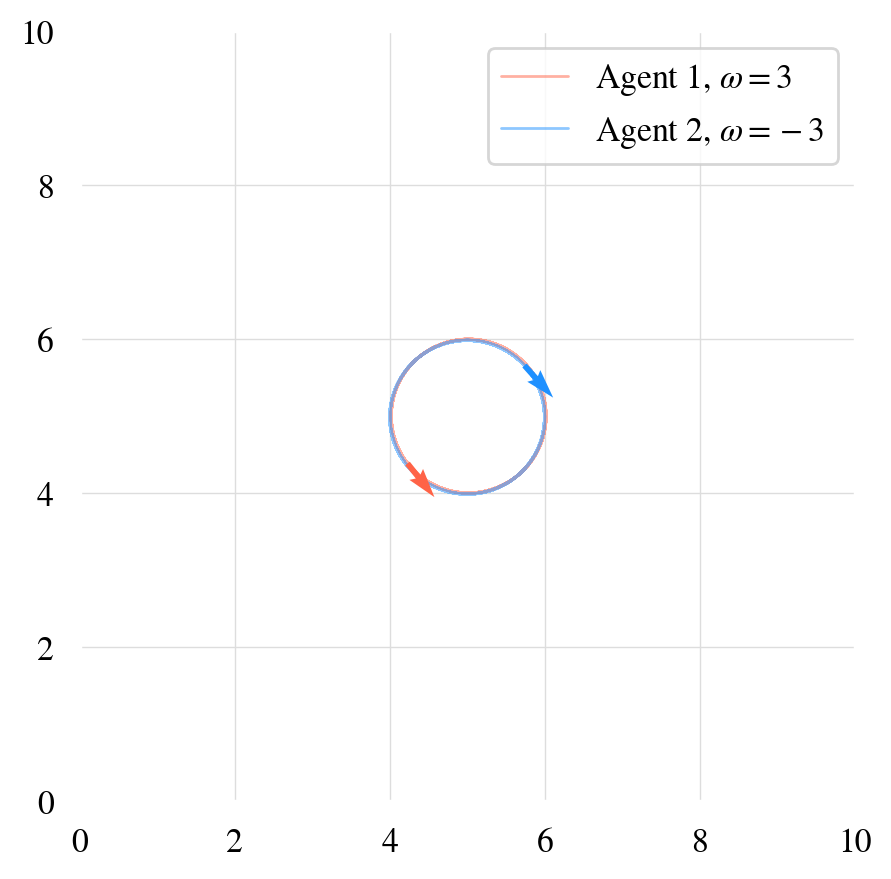
\includegraphics[width=\textwidth]{./figs/noCoupling2particals.png}
	% 	\vspace{-1cm}
	% 	\caption{无耦合}
	% \end{subfigure}

	\begin{subfigure}[b]{0.49\textwidth}
		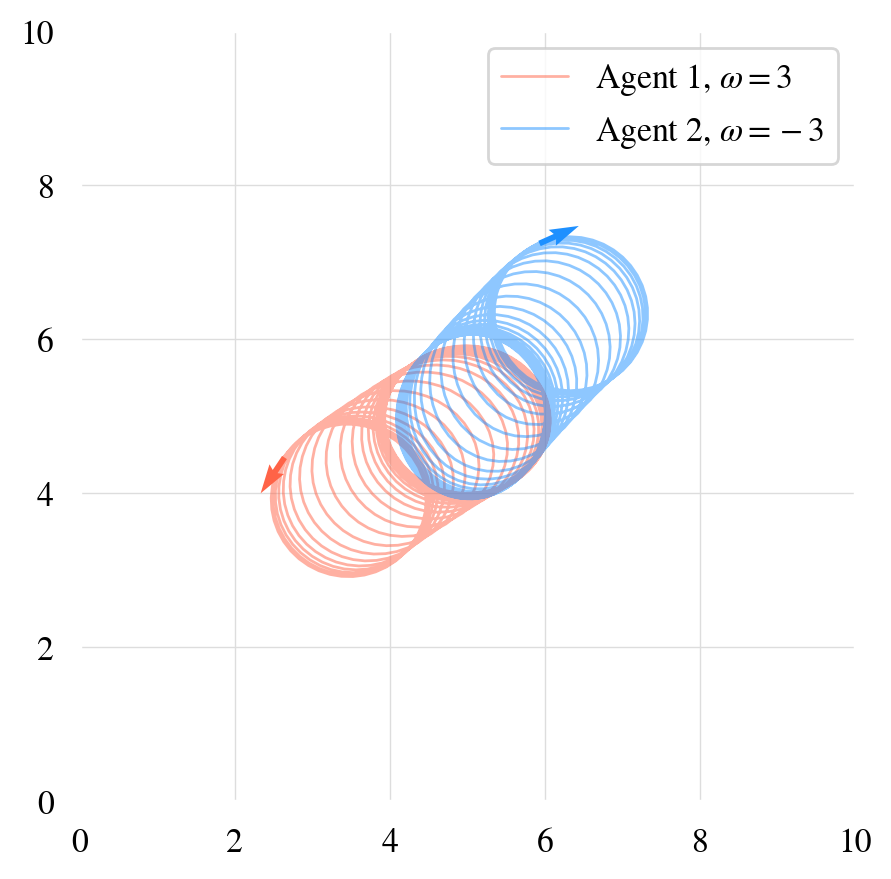
\includegraphics[width=\textwidth]{./figs/diffChir.png}
		\vspace{-1cm}
		\caption{$\omega_1 \cdot \omega_2 < 0$ ($d_0=2$)}
	\end{subfigure}
	% \hfill
	\begin{subfigure}[b]{0.49\textwidth}
		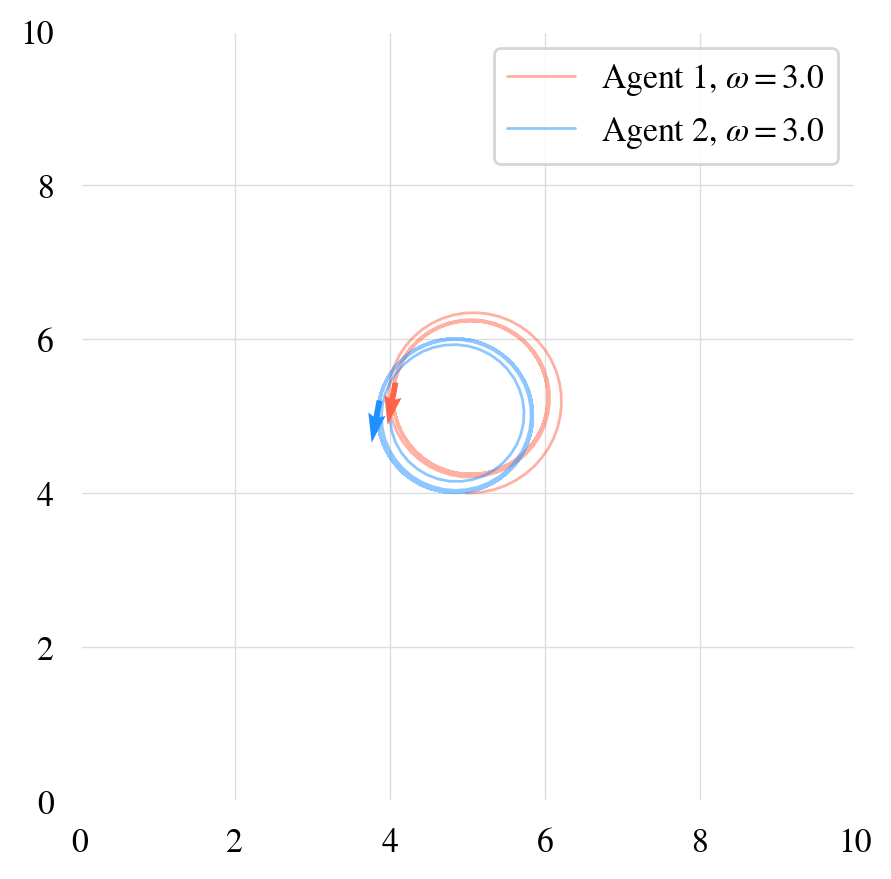
\includegraphics[width=\textwidth]{./figs/sameChir.png}
		\vspace{-1cm}
		\caption{$\omega_1 \cdot \omega_2 < 0$ ($d_0=2$)}
	\end{subfigure}
	% \hfill
	\begin{subfigure}[b]{0.49\textwidth}
		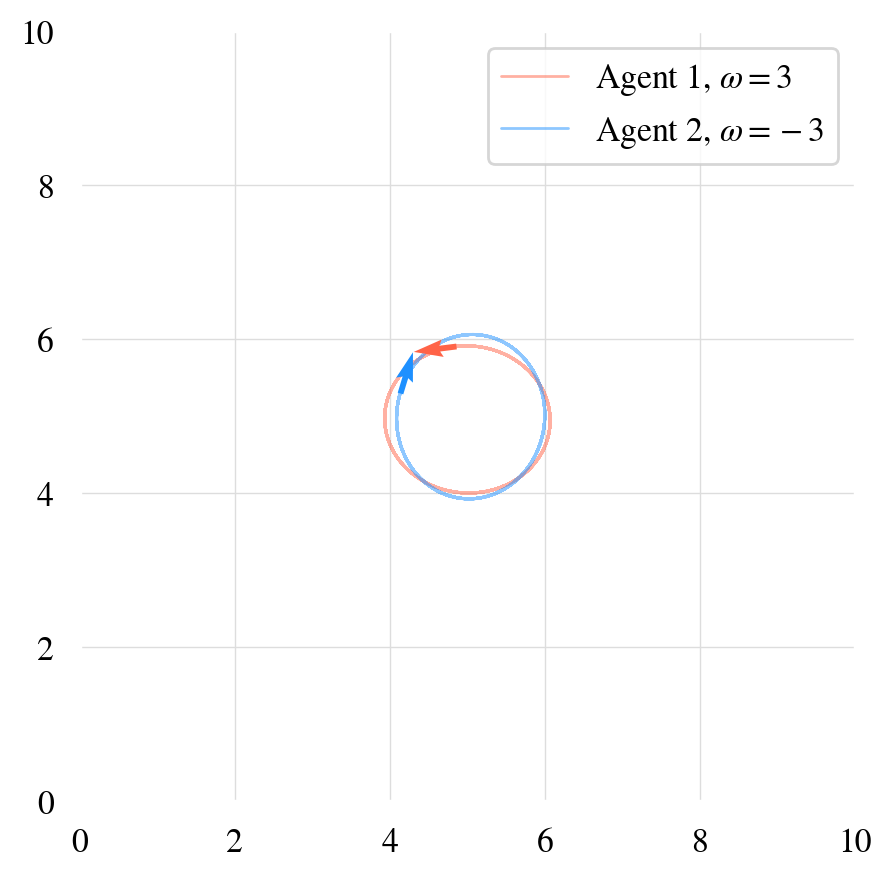
\includegraphics[width=\textwidth]{./figs/diffChirInf.png}
		\vspace{-1cm}
		\caption{$\omega_1 \cdot \omega_2 < 0$ ($d_0=+\infty$)}
	\end{subfigure}
	% \hfill
	\begin{subfigure}[b]{0.49\textwidth}
		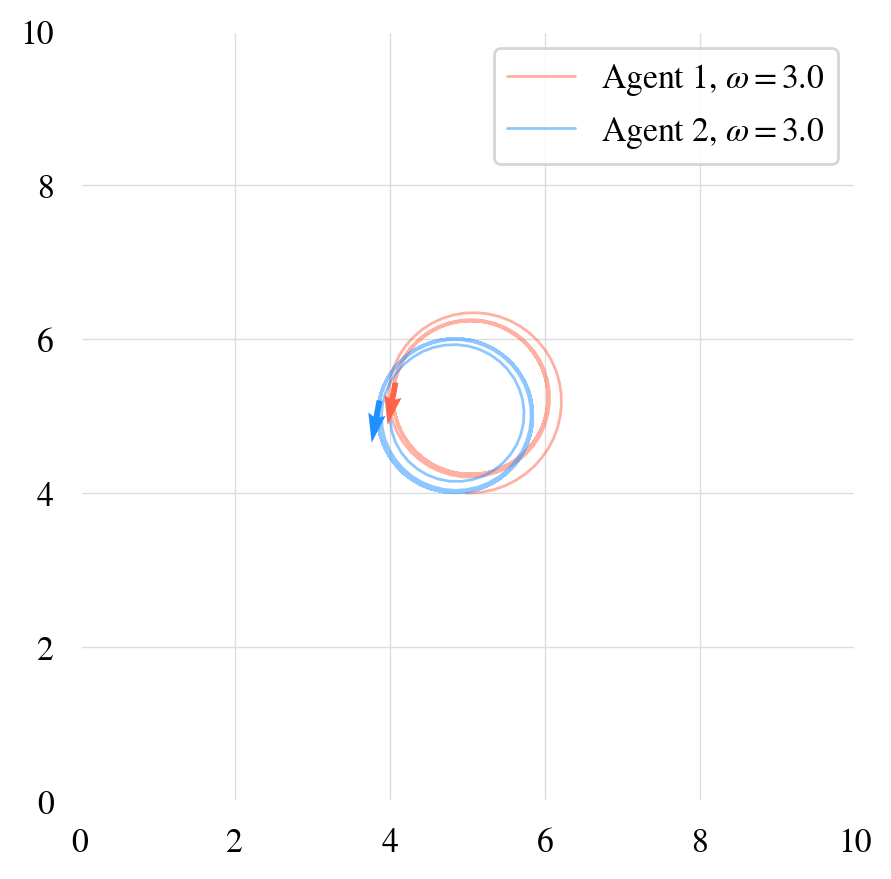
\includegraphics[width=\textwidth]{./figs/sameChirInf.png}
		\vspace{-1cm}
		\caption{$\omega_1 \cdot \omega_2 < 0$ ($d_0=+\infty$)}
	\end{subfigure}
	\caption{同异手性在相同初值条件下的演化结果($\lambda=0.5$)}
	\label{fig:fig2.6.chir}
\end{figure}

\newpage

\begin{figure}[H]
	\centering
	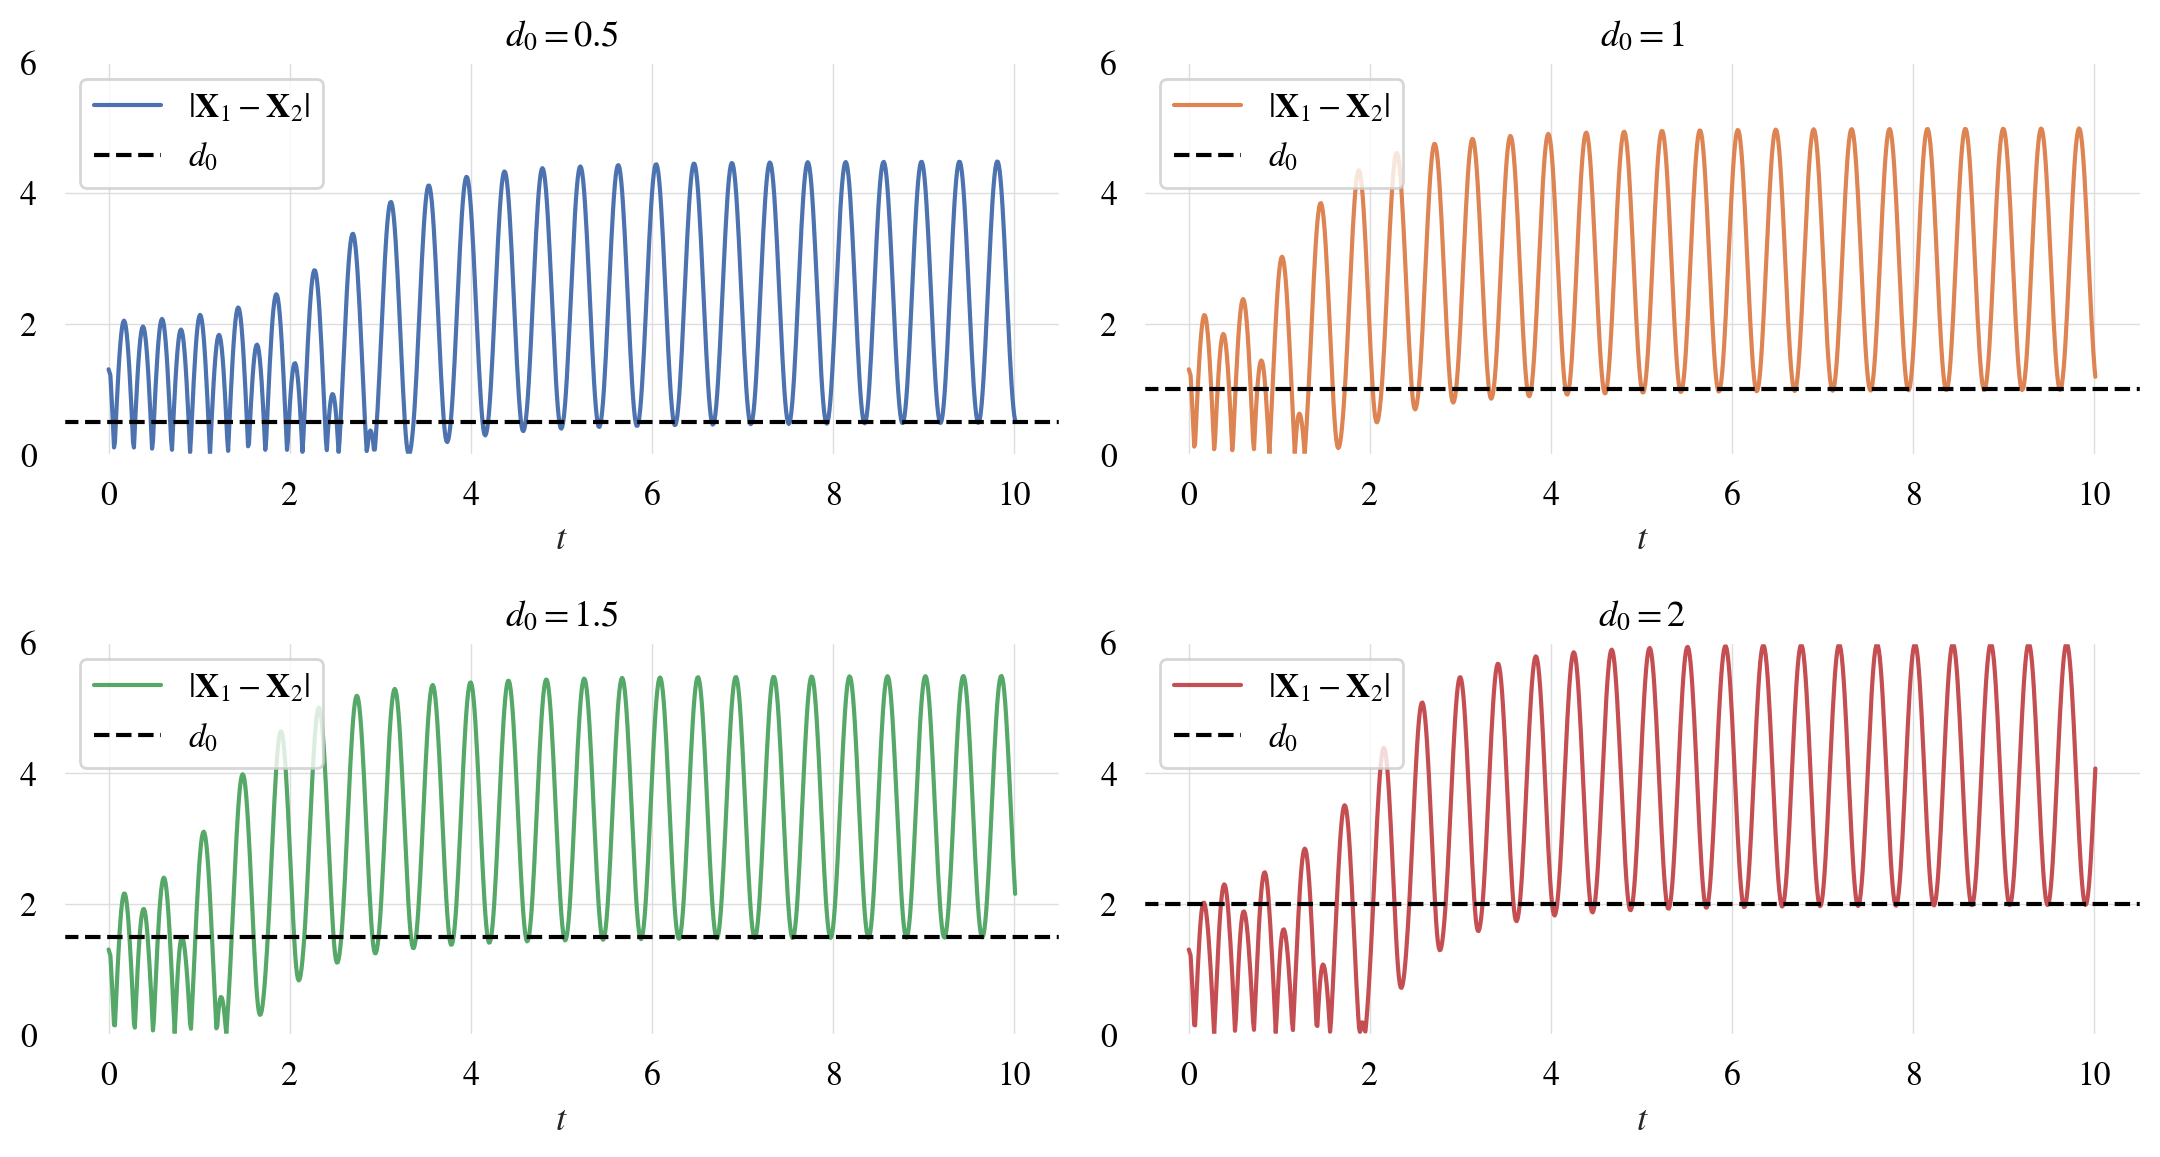
\includegraphics[width=\textwidth]{./figs/2particalDis.png}
	\vspace{-0.5cm}
	\caption{两振子距离的时序变化}
	\label{fig:fig2.6.dis}
\end{figure}

\begin{figure}[H]
	\centering
	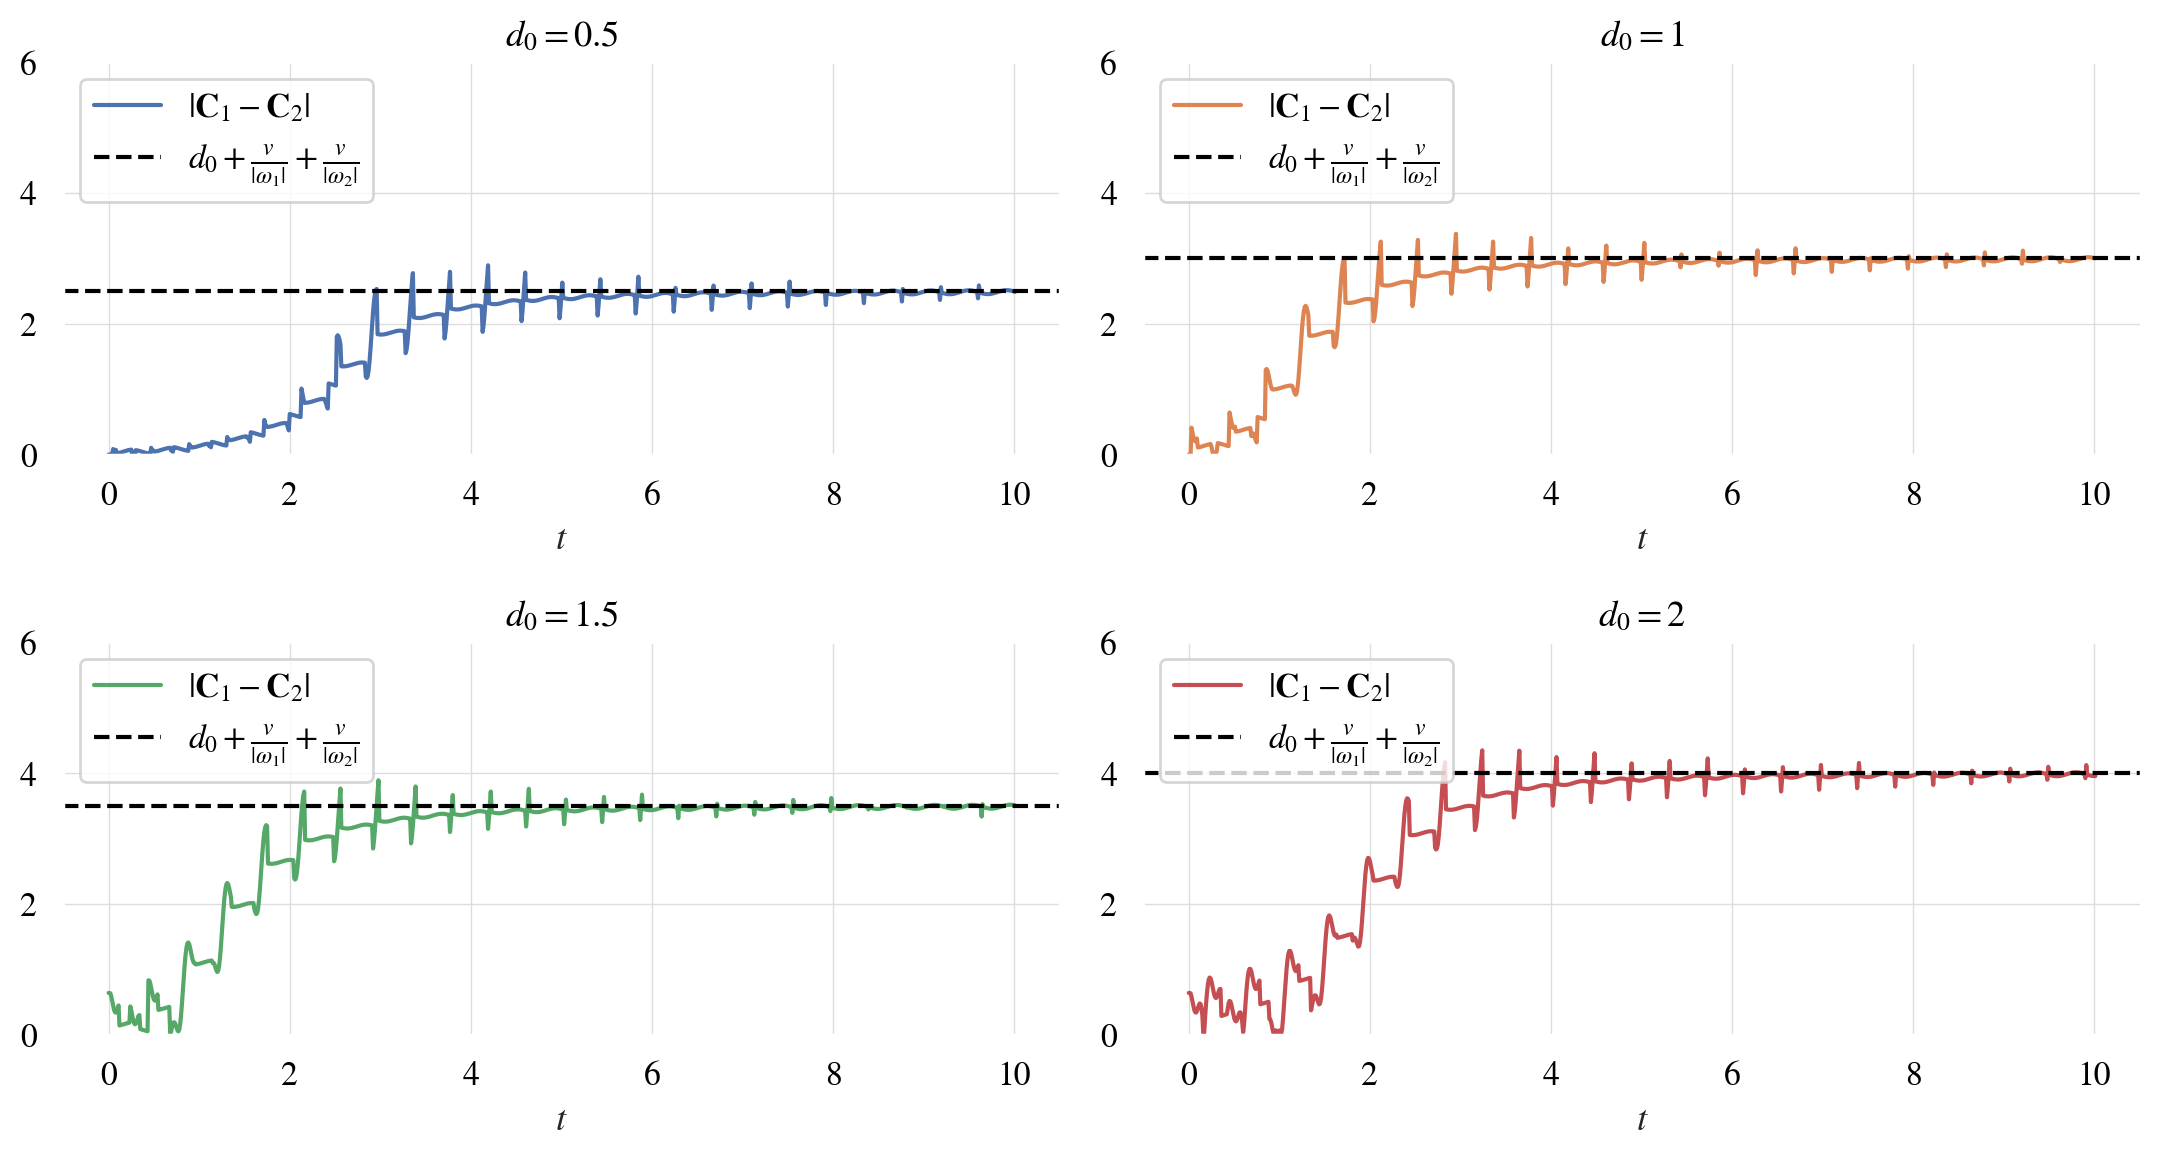
\includegraphics[width=\textwidth]{./figs/2particalCentersDis.png}
	\vspace{-0.5cm}
	\caption{两振子旋转中心距离的时序变化}
	\label{fig:fig2.6.centerDis}
\end{figure}

\newpage
\section{单手性模型环态的细致刻画}

\noindent\textbf{旋转中心邻域内相位同步程度}
$$
S=\frac{1}{N}\sum_{i=1}^N{\left| \frac{1}{N_i}\sum_{j\in C_i}{e^{i\theta _j}} \right|}, C_i=\left\{ j|\bar{d}_{ij}\le d_{th} \right\} 
$$
\vspace{-0.5cm}
\begin{figure}[H]
	\centering
	\begin{subfigure}[b]{0.49\textwidth}
		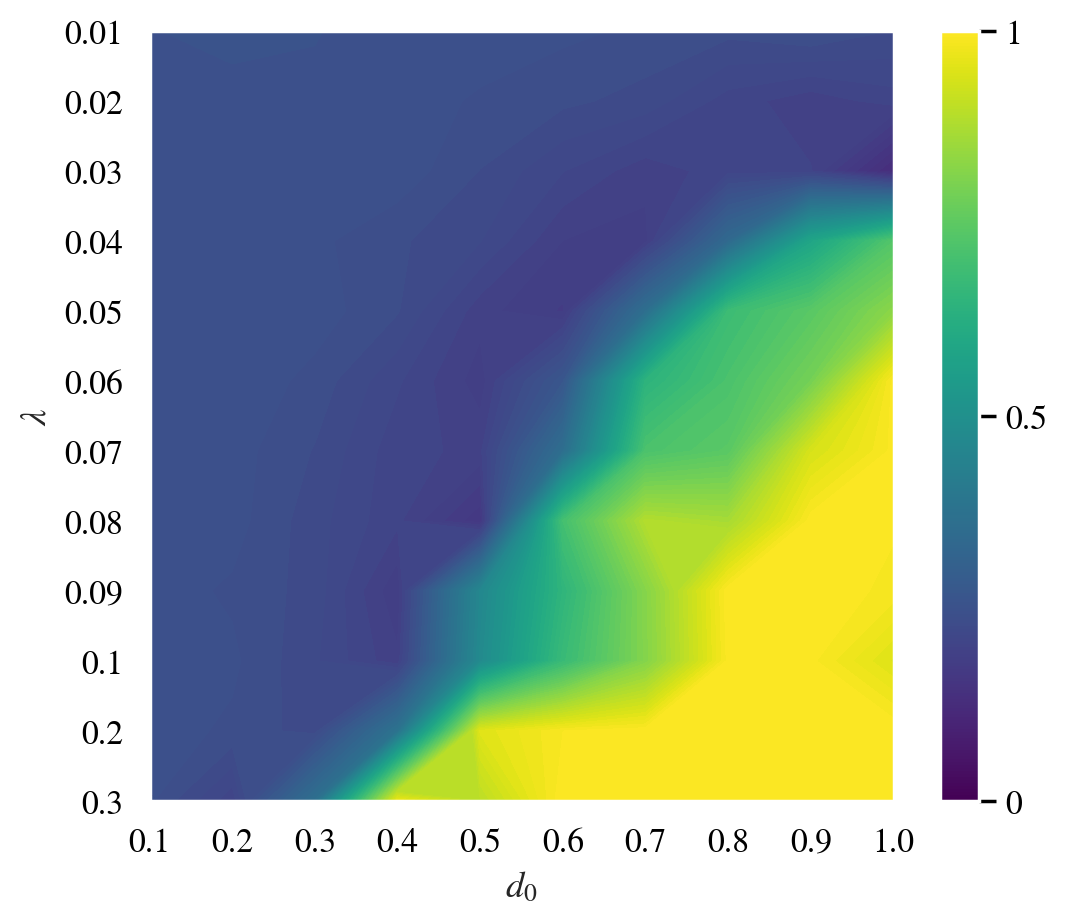
\includegraphics[width=\textwidth]{./figs/limitDisPhaseSyncRing.png}
		\vspace{-1cm}
		\caption{计算结果}
	\end{subfigure}
	% \hfill
	\begin{subfigure}[b]{0.49\textwidth}
		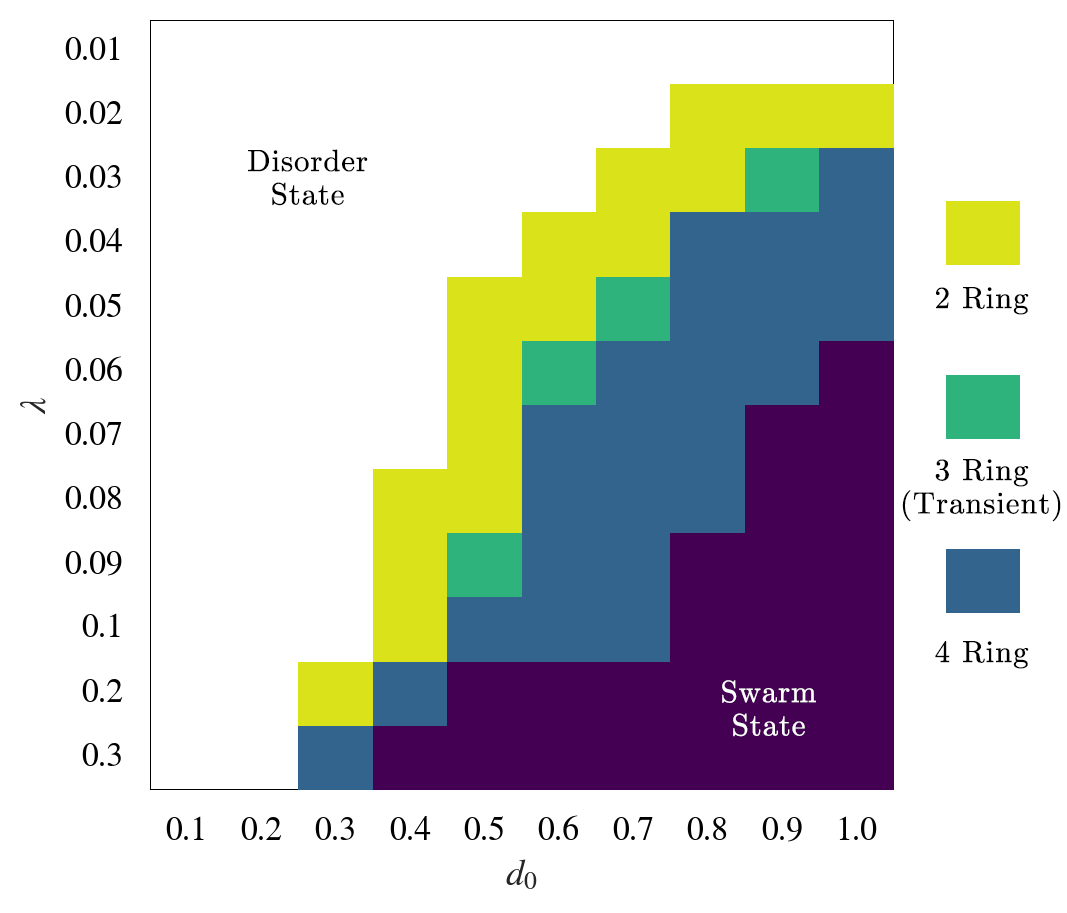
\includegraphics[width=\textwidth]{./figs/subjectiveOpRing.png}
		\vspace{-1cm}
		\caption{主观划分空间状态图}
	\end{subfigure}
	\vspace{-0.5cm}
	\caption{旋转中心邻域内相位同步程度(Single Chirality)}
	\label{fig:fig234c.5.2}
\end{figure}


\noindent\textbf{旋转中心邻域内中心数(截面时序序参量)}

$$
\frac{1}{N}\sum_{i=1}^N{\frac{H\left( d_{th}-\bar{d}_{ij} \right)}{N/2}}=\frac{2}{N^2}\sum_{i=1}^N{H\left( d_{th}-\bar{d}_{ij} \right)}
$$

\vspace{-0.5cm}
\begin{figure}[H]
	\centering
	\begin{subfigure}[b]{0.49\textwidth}
		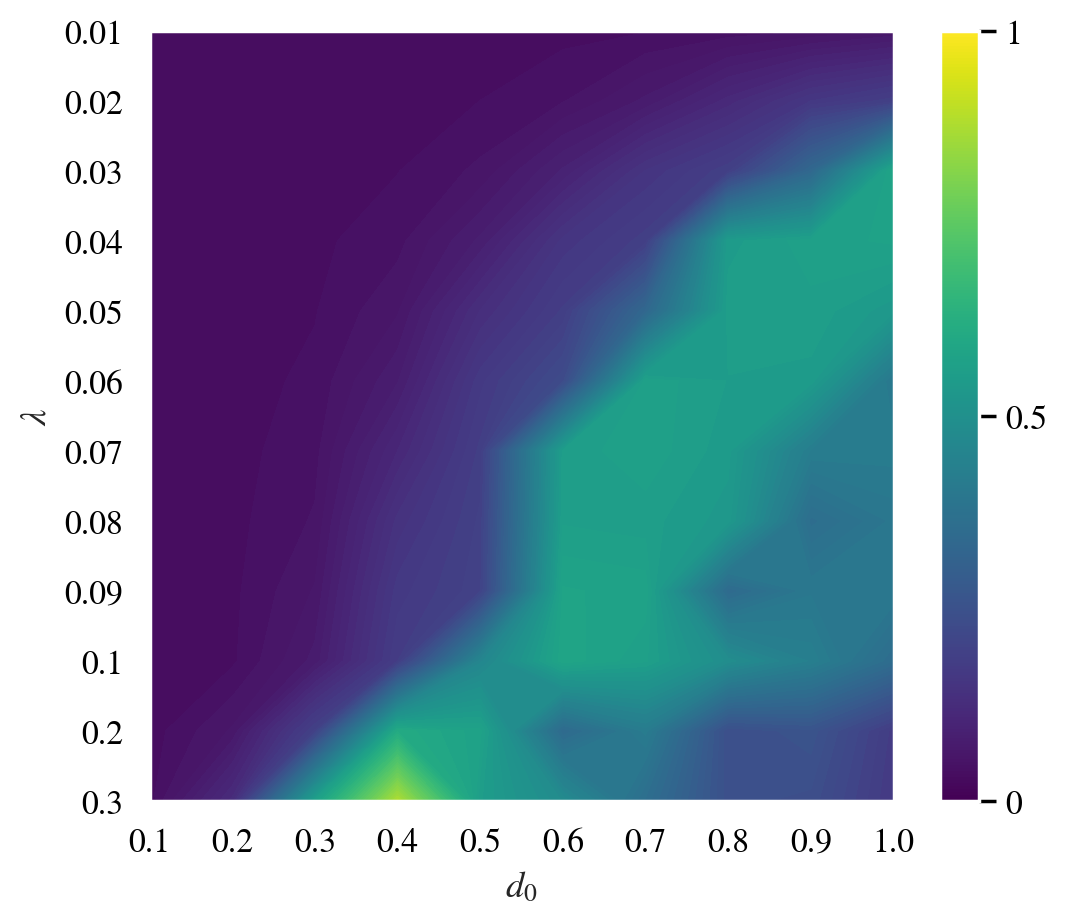
\includegraphics[width=\textwidth]{./figs/nearbyNumsRing.png}
		\vspace{-1cm}
		\caption{计算结果}
		
	\end{subfigure}
	% \hfill
	\begin{subfigure}[b]{0.49\textwidth}
		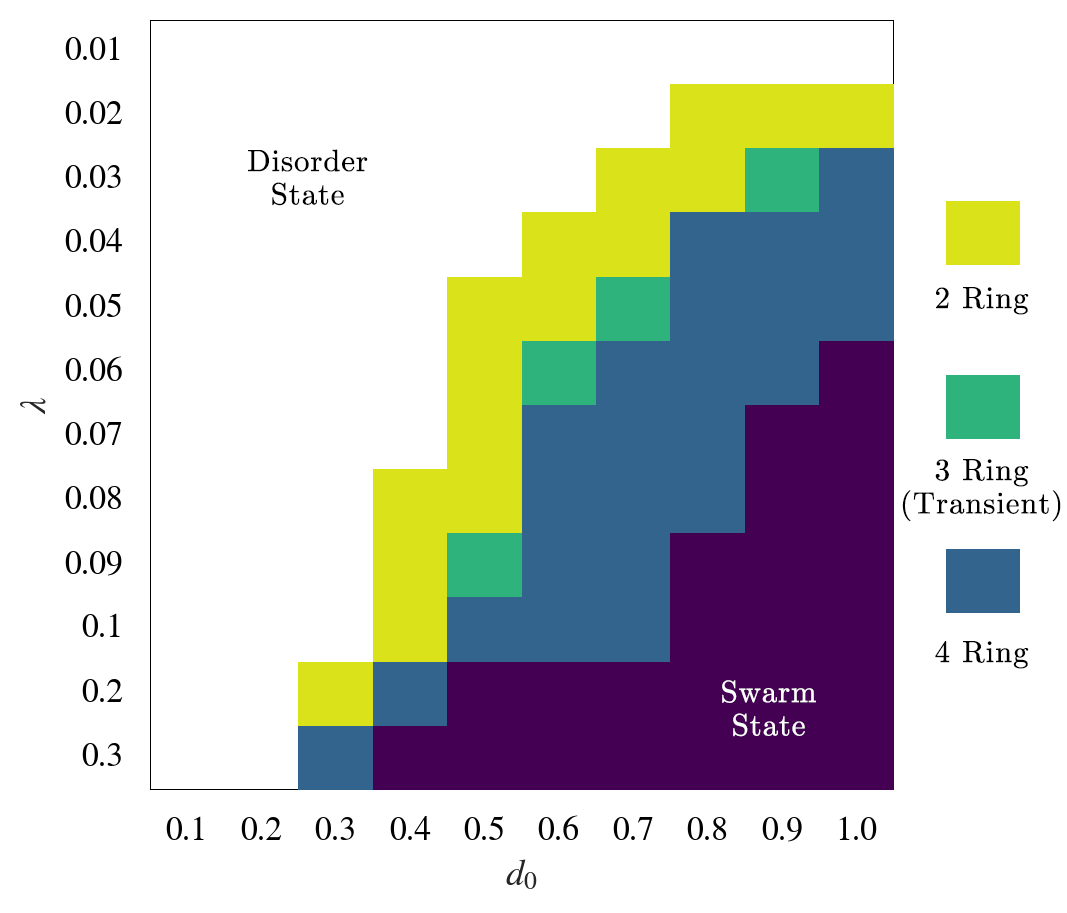
\includegraphics[width=\textwidth]{./figs/subjectiveOpRing.png}
		\vspace{-1cm}
		\caption{主观划分空间状态图}
	\end{subfigure}
	\vspace{-0.5cm}
	\caption{旋转中心邻域内中心数}
	\label{fig:fig234c.7.1}
\end{figure}

% 关于环数的研究, 需注意观察对于各种不同的初值条件的差异. 

% Comments: 
% \begin{itemize}
% 	\item 初值条件对系统的空间集群、相位同步均会产生影响;
% 	\item 当振子空间密集度较高时,初值条件影响应不大;
% 	\item 但密度较低时,初值configuration可能影响较大.
% \end{itemize}



\end{document}